\RequirePackage[l2tabu, orthodox]{nag}

%\documentclass[]{article}
\documentclass[11pt]{scrartcl}
\usepackage[usename, dvipsnames]{xcolor}
\usepackage[pdfencoding=auto]{hyperref}
\usepackage[msc-links]{amsrefs}
\usepackage{cleveref} % use \cref{}, automatically deduces theorem, proposition, etc
\usepackage[mathletters]{ucs}
\usepackage[utf8]{inputenc}
\usepackage[T1]{fontenc}
\usepackage{datetime}

\usepackage{array}
\usepackage{mathtools}
\usepackage{amsmath, amsthm, amssymb, amsfonts, amsxtra, amscd, thmtools}
\let\proof\relax
\let\endproof\relax

% Boxes around theorem environments.
\usepackage[many]{tcolorbox}

\usepackage{color}
%\usepackage{unicode-math}
\usepackage{newunicodechar}
\newunicodechar{ε}{\varepsilon}
\newunicodechar{δ}{\delta}
\newunicodechar{µ}{\mu}
\newunicodechar{→}{\to}
\newunicodechar{≤}{\leq}
\newunicodechar{∈}{\in}
\newunicodechar{⊆}{\subseteq}
\newunicodechar{Λ}{\Lambda}
\newunicodechar{∞}{\infty}
\newunicodechar{×}{\times}
\everymath{\displaystyle}



\usepackage{microtype}
\usepackage[pdfencoding=auto]{hyperref}
\usepackage{bookmark}
\usepackage{booktabs}
\usepackage{todonotes}
\usepackage[msc-links]{amsrefs}
\usepackage{cleveref} % use \cref{}, automatically deduces theorem, proposition, etc
\usepackage{csquotes}
\usepackage{longtable}
\usepackage{tabularx}
\usepackage{bbm}
% Creating multiple types of index
\usepackage{imakeidx}

% Remove indentation for new paragraphs
\usepackage{parskip}
% But leave space before amsthm environments
\makeatletter
\def\thm@space@setup{%
  \thm@preskip=2em
  \thm@postskip=2em
}
\makeatother


\usepackage{stmaryrd}
\usepackage{adjustbox}
\usepackage{centernot}
% \centernot\whatever


% Better indicator function
\usepackage{bbm}
\newcommand{\indic}[1]{\mathbbm{1} \left[ {#1} \right] }

% Highlight quote
\usepackage{environ}
\definecolor{camel}{rgb}{0.76, 0.6, 0.42}
\definecolor{babyblue}{rgb}{0.54, 0.81, 0.94}
\definecolor{block-gray}{gray}{0.85}
\NewEnviron{myblock}
{\colorbox{block-gray}{%
\parbox{\dimexpr\linewidth-2\fboxsep\relax}{%
\small\addtolength{\leftskip}{10mm}
\addtolength{\rightskip}{10mm}
\BODY}}
}
\renewcommand{\quote}{\myblock}
\renewcommand{\endquote}{\endmyblock}

% Nice math font that journals use
%\usepackage[lite]{mtpro2}
%\usepackage{mathrsfs}
%\usepackage{mathptmx}
\usepackage{lmodern}
%\usepackage[sc]{mathpazo}

% Theorem Styles
\usepackage[framemethod=tikz]{mdframed}

\theoremstyle{definition}
\newtheorem{exercise}{Exercise}[section]
\newtheorem{solution}{Solution}

% Theorem Style
\newtheoremstyle{theorem}% name
  {0em}%         Space above, empty = `usual value'
  {1em}%         Space below
  {\normalfont}% Body font
  {\parindent}%         Indent amount (empty = no indent, \parindent = para indent)
  {\bfseries}% Thm head font
  {.}%        Punctuation after thm head
  {\newline}% Space after thm head: \newline = linebreak
  {\thmname{#1}\thmnumber{ #2}\thmnote{\itshape{(#3)}}}%
\theoremstyle{theorem}
\tcolorboxenvironment{theorem}{
  boxrule=0pt,
  boxsep=0pt,
  breakable,
  enhanced jigsaw,
  fonttitle={\large\bfseries},
  opacityback=0.8,
  colframe=cyan,
  borderline west={4pt}{0pt}{orange},
  attach title to upper={}
}
\newtheorem{theorem}{Theorem}[section]

% Proposition Style
\tcolorboxenvironment{proposition}{
  boxrule=1pt,
  boxsep=0pt,
  breakable,
  enhanced jigsaw,
  opacityback=0.0,
  colframe=cyan
}
\newtheorem{proposition}[theorem]{Proposition}
\tcolorboxenvironment{lemma}{
  boxrule=1pt,
  boxsep=0pt,
  breakable,
  enhanced jigsaw,
  opacityback=0.2,
  colframe=cyan
}
\newtheorem{lemma}[theorem]{Lemma}
% Claim
\tcolorboxenvironment{claim}{
  boxrule=1pt,
  boxsep=0pt,
  breakable,
  enhanced jigsaw,
  opacityback=0.2,
  colframe=cyan
}
\newtheorem{claim}[theorem]{Claim}


% Corollary
\tcolorboxenvironment{corollary}{
  colback=cyan,
  boxrule=1pt,
  boxsep=0pt,
  breakable,
  enhanced jigsaw,
  opacityback=0.1,
  colframe=cyan
}
\newtheorem{corollary}[theorem]{Corollary}

% Proof Style
\newtheoremstyle{proof}% name
  {0em}%         Space above, empty = `usual value'
  {2em}%         Space below
  {\normalfont}% Body font
  {\parindent}%         Indent amount (empty = no indent, \parindent = para indent)
  {\itshape}% Thm head font
  {.}%        Punctuation after thm head
  {\newline}% Space after thm head: \newline = linebreak
  {\thmname{#1} \thmnote{\itshape{(#3)}}}%         Thm head spec
\theoremstyle{proof}
\tcolorboxenvironment{proof}{
  colback=camel,
  opacityfill=0.25,
  boxrule=1pt,
  boxsep=0pt,
  breakable,
  enhanced jigsaw
}
\newtheorem*{pf}{Proof}
\newenvironment{proof}
{\pushQED{$\qed$}\pf}
{\par\popQED\endpf}

% Definition Style
\newtheoremstyle{definition}% name
  {0em}%         Space above, empty = `usual value'
  {2em}%         Space below
  {\normalfont}% Body font
  {\parindent}%         Indent amount (empty = no indent, \parindent = para indent)
  {\bfseries}% Thm head font
  {.}%        Punctuation after thm head
  {\newline}% Space after thm head: \newline = linebreak
  {}%         Thm head spec
\theoremstyle{definition}
\tcolorboxenvironment{definition}{
  colback=babyblue,
  boxrule=0pt,
  boxsep=0pt,
  opacityfill=0.45,
  breakable,
  enhanced jigsaw,
  borderline west={4pt}{0pt}{blue},
  colbacktitle={babyblue},
  coltitle={black},
  fonttitle={\large\bfseries},
  attach title to upper={},
}
\newtheorem{definition}{Definition}[theorem]

% Break Environment
\makeatletter
\newtheoremstyle{break}% name
  {}%         Space above, empty = `usual value'
  {2em}%         Space below
  {
    \addtolength{\@totalleftmargin}{2.5em}
    \addtolength{\linewidth}{-2.5em}
    \parshape 1 2.5em \linewidth
  }% Body font
  {}%         Indent amount (empty = no indent, \parindent = para indent)
  {\bfseries}% Thm head font
  {.}%        Punctuation after thm head
  {\newline}% Space after thm head: \newline = linebreak
  {}%         Thm head spec
\makeatother

\theoremstyle{break}
\newtheorem{example}{Example}[section]

% Problem Style
\newtheoremstyle{problem} % name
  {0em}                   % Space above, empty = `usual value'
  {2em}                   % Space below
  {\normalfont}           % Body font
  {\parindent}            % Indent amount (empty = no indent, \parindent = para indent)
  {\itshape}              % Thm head font
  {}                      % Punctuation after thm head
  {\newline}              % Space after thm head: \newline = linebreak
  {\thmnote{\itshape{(#3)}}}     % Thm head spec
\theoremstyle{problem}
\tcolorboxenvironment{problem}{
  boxrule=1pt,
  boxsep=0pt,
  breakable,
  enhanced jigsaw,
  opacityback=0.0,
  colframe=cyan
}
\newtheorem{problem}{Problem}


%Pagination stuff.
\setlength{\topmargin}{-.3 in}
\setlength{\oddsidemargin}{0in}
\setlength{\evensidemargin}{0in}
\setlength{\textheight}{9.in}
\setlength{\textwidth}{6.5in}
% \pagestyle{empty} %removes page numbers.

% Inkscape figures from Vim
\usepackage{import}
\usepackage{pdfpages}
\usepackage{transparent}

\newcommand{\incfig}[1]{%
    \def\svgwidth{\columnwidth}
    \import{./figures/}{#1.pdf_tex}
}
%\pdfsuppresswarningpagegroup=1

% Pandoc-specific fixes
\providecommand{\tightlist}{%
  \setlength{\itemsep}{0pt}\setlength{\parskip}{0pt}}

% Tikz and Graphics
\usepackage{amscd}
\usepackage{tikz}
\usetikzlibrary{arrows, arrows.meta, cd, fadings, patterns, calc, decorations.markings, matrix, positioning}
\tikzfading[name=fade out, inner color=transparent!0, outer color=transparent!100]
\usepackage{pgfplots}
\pgfplotsset{compat=1.16}
\usepackage[inline]{asymptote}
\usepackage{tikz-layers}

%\usepackage{nath}
%\delimgrowth=1
\DeclarePairedDelimiter\qty{(}{)}

% Major Macros
\usepackage{graphicx}
\usepackage{float}
\DeclareFontFamily{U}{mathx}{\hyphenchar\font45}
\DeclareFontShape{U}{mathx}{m}{n}{
      <5> <6> <7> <8> <9> <10>
      <10.95> <12> <14.4> <17.28> <20.74> <24.88>
      mathx10
      }{}
\DeclareSymbolFont{mathx}{U}{mathx}{m}{n}
\DeclareMathSymbol{\bigtimes}{1}{mathx}{"91}

% Wide tikz equations
\newsavebox{\wideeqbox}
\newenvironment{wideeq}
  {\begin{displaymath}\begin{lrbox}{\wideeqbox}$\displaystyle}
  {$\end{lrbox}\makebox[0pt]{\usebox{\wideeqbox}}\end{displaymath}}



% Fancy chapter headers and footers
\usepackage{fancyhdr}

\pagestyle{fancy}
\fancyhf{}
\fancyhead[LE,RO]{\title}
\fancyhead[RE,LO]{\rightmark}
\fancyfoot[CE,CO]{\leftmark}
\fancyfoot[LE,RO]{\thepage}

\renewcommand{\headrulewidth}{2pt}
\renewcommand{\footrulewidth}{1pt}

% List of Theorems Attempt
\usepackage{etoolbox}
\makeatletter
\patchcmd\thmtlo@chaptervspacehack
  {\addtocontents{loe}{\protect\addvspace{10\p@}}}
  {\addtocontents{loe}{\protect\thmlopatch@endchapter\protect\thmlopatch@chapter{\thechapter}}}
  {}{}
\AtEndDocument{\addtocontents{loe}{\protect\thmlopatch@endchapter}}
\long\def\thmlopatch@chapter#1#2\thmlopatch@endchapter{%
  \setbox\z@=\vbox{#2}%
  \ifdim\ht\z@>\z@
    \hbox{\bfseries\chaptername\ #1}\nobreak
    #2
    \addvspace{10\p@}
  \fi
}
\def\thmlopatch@endchapter{}

\makeatother
\renewcommand{\thmtformatoptarg}[1]{ -- #1}
%\renewcommand{\listtheoremname}{List of definitions}

\newcommand{\ext}{\operatorname{Ext}}
\newcommand{\Ext}{\operatorname{Ext}}
\def\Endo{\operatorname{End}}
\def\Ind{\operatorname{Ind}}
\def\ind{\operatorname{Ind}}
\def\coind{\operatorname{Coind}}
\def\Res{\operatorname{Res}}
\def\Hol{\operatorname{Hol}}
\def\res{\operatorname{Res}}
\def\endo{\operatorname{End}}
\def\ind{\operatorname{Ind}}
\renewcommand{\AA}[0]{{\mathbb{A}}}
\DeclareMathOperator{\Exists}{\exists}
\DeclareMathOperator{\Forall}{\forall}
\newcommand{\Af}[0]{{\mathbb{A}}}
\newcommand{\CC}[0]{{\mathbb{C}}}
\newcommand{\CP}[0]{{\mathbb{CP}}}
\newcommand{\DD}[0]{{\mathbb{D}}}
\newcommand{\FF}[0]{{\mathbb{F}}}
\newcommand{\GF}[0]{{\mathbb{GF}}}
\newcommand{\GG}[0]{{\mathbb{G}}}
\newcommand{\HH}[0]{{\mathbb{H}}}
\newcommand{\HP}[0]{{\mathbb{HP}}}
\newcommand{\KK}[0]{{\mathbb{K}}}
\newcommand{\kk}[0]{{\Bbbk}}
\newcommand{\bbm}[0]{{\mathbb{M}}}
\newcommand{\NN}[0]{{\mathbb{N}}}
\newcommand{\OP}[0]{{\mathbb{OP}}}
\newcommand{\PP}[0]{{\mathbb{P}}}
\newcommand{\QQ}[0]{{\mathbb{Q}}}
\newcommand{\RP}[0]{{\mathbb{RP}}}
\newcommand{\RR}[0]{{\mathbb{R}}}
\newcommand{\SpSp}[0]{{\mathbb{S}}}
\renewcommand{\SS}[0]{{\mathbb{S}}}
\newcommand{\TT}[0]{{\mathbb{T}}}
\newcommand{\ZZ}[0]{{\mathbb{Z}}}
\newcommand{\ZnZ}[0]{\mathbb{Z}/n\mathbb{Z}}
\newcommand{\ZpZ}[0]{\mathbb{Z}/p\mathbb{Z}}
\newcommand{\Qp}[0]{\mathbb{Q}_{(p)}}
\newcommand{\Zp}[0]{\mathbb{Z}_{(p)}}
\newcommand{\Arg}[0]{\mathrm{Arg}}
\newcommand{\PGL}[0]{\mathrm{PGL}}
\newcommand{\GL}[0]{\mathrm{GL}}
\newcommand{\Gl}[0]{\mathrm{GL}}
\newcommand{\gl}[0]{\mathrm{GL}}
\newcommand{\mat}[0]{\mathrm{Mat}}
\newcommand{\Mat}[0]{\mathrm{Mat}}
\newcommand{\Rat}[0]{\mathrm{Rat}}
\newcommand{\Perv}[0]{\mathrm{Perv}}
\newcommand{\Gal}[0]{\mathrm{Gal}}
\newcommand{\Hilb}[0]{\mathrm{Hilb}}
\newcommand{\Quot}[0]{\mathrm{Quot}}
\newcommand{\Art}[0]{\mathrm{Art}}
\newcommand{\red}[0]{\mathrm{red}}
\newcommand{\alg}[0]{\mathrm{alg}}
\newcommand{\Pic}[0]{{\mathrm{Pic}~}}
\newcommand{\lcm}[0]{\mathrm{lcm}}
\newcommand{\maps}[0]{\mathrm{Maps}}
\newcommand{\maxspec}[0]{{\mathrm{maxSpec}~}}
\newcommand{\Tr}[0]{\mathrm{Tr}}
\newcommand{\adj}[0]{\mathrm{adj}}
\newcommand{\ad}[0]{\mathrm{ad}~}
\newcommand{\ann}[0]{\mathrm{Ann}}
\newcommand{\Ann}[0]{\mathrm{Ann}}
\newcommand{\arcsec}[0]{\mathrm{arcsec}}
\newcommand{\ch}[0]{\mathrm{char}~}
\newcommand{\Sp}[0]{{\mathrm{Sp}}}
\newcommand{\syl}[0]{{\mathrm{Syl}}}
\newcommand{\txand}[0]{{\text{ and }}}
\newcommand{\codim}[0]{\mathrm{codim}}
\newcommand{\txor}[0]{{\text{ or }}}
\newcommand{\txt}[1]{{\text{ {#1} }}}
\newcommand{\Gr}[0]{{\text{Gr}}}
\newcommand{\Aut}[0]{{\mathrm{Aut}}}
\newcommand{\aut}[0]{\mathrm{Aut}}
\newcommand{\Inn}[0]{{\mathrm{Inn}}}
\newcommand{\Out}[0]{{\mathrm{Out}}}
\newcommand{\mltext}[1]{\left\{\begin{array}{c}#1\end{array}\right\}}
\newcommand{\Fun}[0]{{\text{Fun}}}
\newcommand{\SL}[0]{{\text{SL}}}
\newcommand{\PSL}[0]{{\text{PSL}}}
\newcommand{\SO}[0]{{\text{SO}}}
\newcommand{\SU}[0]{{\text{SU}}}
\newcommand{\SP}[0]{{\text{SP}}}
\newcommand{\per}[0]{{\text{Per}}}
\newcommand{\loc}[0]{{\text{loc}}}
\newcommand{\Top}[0]{{\text{Top}}}
\newcommand{\Sch}[0]{{\text{Sch}}}
\newcommand{\sch}[0]{{\text{Sch}}}
\newcommand{\Set}[0]{{\text{Set}}}
\newcommand{\Sets}[0]{{\text{Set}}}
\newcommand{\Grp}[0]{{\text{Grp}}}
\newcommand{\Groups}[0]{{\text{Groups}}}
\newcommand{\Homeo}[0]{{\text{Homeo}}}
\newcommand{\Diffeo}[0]{{\text{Diffeo}}}
\newcommand{\MCG}[0]{{\text{MCG}}}
\newcommand{\set}[0]{{\text{Set}}}
\newcommand{\Tor}[0]{\text{Tor}}
\newcommand{\sets}[0]{{\text{Set}}}
\newcommand{\Sm}[0]{{\text{Sm}_k}}
\newcommand{\orr}[0]{{\text{ or }}}
\newcommand{\annd}[0]{{\text{ and }}}
\newcommand{\bung}[0]{\text{Bun}_G}
\newcommand{\const}[0]{{\text{const.}}}
\newcommand{\disc}[0]{{\text{disc}}}
\newcommand{\op}[0]{^\text{op}}
\newcommand{\id}[0]{\text{id}}
\newcommand{\im}[1]{\mathrm{im}({#1})}
\newcommand{\pt}[0]{{\{\text{pt}\}}}
\newcommand{\sep}[0]{^\text{sep}}
% \newcommand{\st}[0]{~{\text{s.t.}}~}
\newcommand{\tors}[0]{{\text{tors}}}
\newcommand{\tor}[0]{\text{Tor}}
\newcommand{\height}[0]{\text{ht}}
\newcommand{\cpt}[0]{\text{compact}}
\newcommand{\abs}[1]{{\left\lvert {#1} \right\rvert}}
\newcommand{\stack}[1]{\mathclap{\substack{ #1 }}} 
\newcommand{\qtext}[1]{{\quad \text{#1} \quad}}
\newcommand{\qst}[0]{{\quad \text{such that} \quad}}
\newcommand{\actsonl}[0]{\curvearrowleft}
\newcommand{\actson}[0]{\curvearrowright}
\newcommand{\bd}[0]{{\del}}
\newcommand{\bigast}[0]{{\mathop{\Large \ast}}}
\newcommand{\coker}[0]{\operatorname{coker}}
\newcommand{\cok}[0]{\operatorname{coker}}
\newcommand{\conjugate}[1]{{\overline{{#1}}}}
\newcommand{\converges}[1]{\overset{#1}}
\newcommand{\correspond}[1]{\theset{\substack{#1}}}
\newcommand{\cross}[0]{\times}
\newcommand{\by}[0]{\times}
\newcommand{\dash}[0]{{\hbox{-}}}
\newcommand{\dd}[2]{{\frac{\partial #1}{\partial #2}\,}}
\newcommand{\definedas}[0]{\coloneqq}
\newcommand{\da}[0]{\coloneqq}
\newcommand{\del}[0]{{\partial}}
\newcommand{\directlim}[0]{\varinjlim}
\newcommand{\disjoint}[0]{{\coprod}}
\newcommand{\divides}[0]{{~\Bigm|~}}
\newcommand{\dual}[0]{^\vee}
\newcommand{\sm}[0]{\setminus}
\newcommand{\smz}[0]{\setminus\theset{0}}
\newcommand{\eps}[0]{\varepsilon}
\newcommand{\equalsbecause}[1] {\stackrel{\mathclap{\scriptscriptstyle{#1}}}{=}}
\newcommand{\floor}[1]{{\left\lfloor #1 \right\rfloor}}
\DeclarePairedDelimiter{\ceil}{\lceil}{\rceil}
\newcommand{\from}[0]{\leftarrow}
\newcommand{\tofrom}[0]{\leftrightarrows}
\newcommand{\up}[0]{\uparrow}
\newcommand{\generators}[1]{\left\langle{#1}\right\rangle}
\newcommand{\gs}[1]{\left\langle{#1}\right\rangle}
\newcommand{\homotopic}[0]{\simeq}
\newcommand{\injectivelim}[0]{\varinjlim}
\newcommand{\injects}[0]{\hookrightarrow}
\newcommand{\inner}[2]{{\left\langle {#1},~{#2} \right\rangle}}
\newcommand{\union}[0]{\cup}
\newcommand{\Union}[0]{\bigcup}
\newcommand{\intersect}[0]{\cap}
\newcommand{\Intersect}[0]{\bigcap}
\newcommand{\into}[0]{\to}
\newcommand{\inverselim}[0]{\varprojlim}
\newcommand{\inv}[0]{^{-1}}
\newcommand{\mfa}[0]{{\mathfrak{a}}}
\newcommand{\mfb}[0]{{\mathfrak{b}}}
\newcommand{\mfc}[0]{{\mathfrak{c}}}
\newcommand{\mff}[0]{{\mathfrak{f}}}
\newcommand{\mfi}[0]{{\mathfrak{I}}}
\newcommand{\mfm}[0]{{\mathfrak{m}}}
\newcommand{\mfn}[0]{{\mathfrak{n}}}
\newcommand{\mfp}[0]{{\mathfrak{p}}}
\newcommand{\mfq}[0]{{\mathfrak{q}}}
\newcommand{\mfr}[0]{{\mathfrak{r}}}
\newcommand{\lieb}[0]{{\mathfrak{b}}}
\newcommand{\liegl}[0]{{\mathfrak{gl}}}
\newcommand{\lieg}[0]{{\mathfrak{g}}}
\newcommand{\lieh}[0]{{\mathfrak{h}}}
\newcommand{\lien}[0]{{\mathfrak{n}}}
\newcommand{\liesl}[0]{{\mathfrak{sl}}}
\newcommand{\lieso}[0]{{\mathfrak{so}}}
\newcommand{\liesp}[0]{{\mathfrak{sp}}}
\newcommand{\lieu}[0]{{\mathfrak{u}}}
\newcommand{\nilrad}[0]{{\mathfrak{N}}}
\newcommand{\jacobsonrad}[0]{{\mathfrak{J}}}
\newcommand{\mm}[0]{{\mathfrak{m}}}
\newcommand{\pr}[0]{{\mathfrak{p}}}
\newcommand{\mapsvia}[1]{\xrightarrow{#1}}
\newcommand{\kx}[1]{k[x_1, \cdots, x_{#1}]}
\newcommand{\MM}[0]{{\mathcal{M}}}
\newcommand{\OO}[0]{{\mathcal{O}}}
\newcommand{\imaginarypart}[1]{{\mathcal{Im}({#1})}}
\newcommand{\mca}[0]{{\mathcal{A}}}
\newcommand{\mcb}[0]{{\mathcal{B}}}
\newcommand{\mcc}[0]{{\mathcal{C}}}
\newcommand{\mcd}[0]{{\mathcal{D}}}
\newcommand{\mce}[0]{{\mathcal{E}}}
\newcommand{\mcf}[0]{{\mathcal{F}}}
\newcommand{\mcg}[0]{{\mathcal{G}}}
\newcommand{\mch}[0]{{\mathcal{H}}}
\newcommand{\mci}[0]{{\mathcal{I}}}
\newcommand{\mcj}[0]{{\mathcal{J}}}
\newcommand{\mck}[0]{{\mathcal{K}}}
\newcommand{\mcl}[0]{{\mathcal{L}}}
\newcommand{\mcm}[0]{{\mathcal{M}}}
\newcommand{\mcp}[0]{{\mathcal{P}}}
\newcommand{\mcs}[0]{{\mathcal{S}}}
\newcommand{\mct}[0]{{\mathcal{T}}}
\newcommand{\mcu}[0]{{\mathcal{U}}}
\newcommand{\mcv}[0]{{\mathcal{V}}}
\newcommand{\mcx}[0]{{\mathcal{X}}}
\newcommand{\mcz}[0]{{\mathcal{Z}}}
\newcommand{\cl}[0]{\mathrm{cl}}
\newcommand{\trdeg}[0]{\mathrm{trdeg}}
\newcommand{\dist}[0]{\mathrm{dist}}
\newcommand{\Dist}[0]{\mathrm{Dist}}
\newcommand{\crit}[0]{\mathrm{crit}}
\newcommand{\diam}[0]{{\mathrm{diam}}}
\newcommand{\gal}[0]{\mathrm{Gal}}
\newcommand{\diff}[0]{\mathrm{Diff}}
\newcommand{\diag}[0]{\mathrm{diag}}
\newcommand{\soc}[0]{\mathrm{Soc}\,}
\newcommand{\hd}[0]{\mathrm{Head}\,}
\newcommand{\grad}[0]{\mathrm{grad}~}
\newcommand{\hilb}[0]{\mathrm{Hilb}}
\newcommand{\minpoly}[0]{{\mathrm{minpoly}}}
\newcommand{\Hom}[0]{{\mathrm{Hom}}}
\newcommand{\Map}[0]{{\mathrm{Map}}}
\newcommand{\multinomial}[1]{\left(\!\!{#1}\!\!\right)}
\newcommand{\nil}[0]{{\mathrm{nil}}}
\newcommand{\normalneq}{\mathrel{\reflectbox{$\trianglerightneq$}}}
\newcommand{\normal}[0]{{~\trianglelefteq~}}
\newcommand{\norm}[1]{{\left\lVert {#1} \right\rVert}}
\newcommand{\pnorm}[2]{{\left\lVert {#1} \right\rVert}_{#2}}
\newcommand{\notdivides}[0]{\nmid}
\newcommand{\onto}[0]{\twoheadhthtarrow}
\newcommand{\ord}[0]{{\mathrm{Ord}}}
\newcommand{\pic}[0]{{\mathrm{Pic}~}}
\newcommand{\projectivelim}[0]{\varprojlim}
\newcommand{\rad}[0]{{\mathrm{rad}~}}
\newcommand{\ralg}[0]{\mathrm{R-alg}}
\newcommand{\kalg}[0]{k\dash\mathrm{alg}}
\newcommand{\rank}[0]{\operatorname{rank}}
\newcommand{\realpart}[1]{{\mathcal{Re}({#1})}}
\newcommand{\Log}[0]{\mathrm{Log}}
\newcommand{\reg}[0]{\mathrm{Reg}}
\newcommand{\restrictionof}[2]{{\left.{#1}\right|_{#2}}}
\newcommand{\ro}[2]{{\left.{#1}\right|_{#2}}}
\newcommand{\rk}[0]{{\mathrm{rank}}}
\newcommand{\evalfrom}[0]{\Big|}
\newcommand{\rmod}[0]{{R\dash\mathrm{mod}}}
\newcommand{\Mod}[0]{{\mathrm{Mod}}}
\newcommand{\rotate}[2]{{\style{display: inline-block; transform: rotate(#1deg)}{#2}}}
\newcommand{\selfmap}[0]{{\circlearrowleft}}
\newcommand{\semidirect}[0]{\rtimes}
\newcommand{\sgn}[0]{\mathrm{sgn}}
\newcommand{\sign}[0]{\mathrm{sign}}
\newcommand{\spanof}[0]{{\mathrm{span}}}
\newcommand{\spec}[0]{\mathrm{Spec}\,}
\newcommand{\mspec}[0]{\mathrm{mSpec}~}
\newcommand{\stab}[0]{{\mathrm{Stab}}}
\newcommand{\stirlingfirst}[2]{\genfrac{[}{]}{0pt}{}{#1}{#2}}
\newcommand{\stirling}[2]{\genfrac\{\}{0pt}{}{#1}{#2}}
\newcommand{\strike}[1]{{\enclose{horizontalstrike}{#1}}}
\newcommand{\suchthat}[0]{{~\mathrel{\Big|}~}}
\newcommand{\st}[0]{{~\mathrel{\Big|}~}}
\newcommand{\supp}[0]{{\mathrm{supp}}}
\newcommand{\surjects}[0]{\twoheadrightarrow}
\newcommand{\sym}[0]{\mathrm{Sym}}
\newcommand{\tensor}[0]{\otimes}
\newcommand{\connectsum}[0]{\mathop{\Large \#}}
\newcommand{\theset}[1]{\left\{{#1}\right\}}
\newcommand{\ts}[1]{\left\{{#1}\right\}}
\newcommand{\gens}[1]{\left\langle{#1}\right\rangle}
\newcommand{\thevector}[1]{{\left[ {#1} \right]}}
\newcommand{\tv}[1]{{\left[ {#1} \right]}}
\newcommand{\too}[1]{{\xrightarrow{#1}}}
\newcommand{\transverse}[0]{\pitchfork}
\newcommand{\trianglerightneq}{\mathrel{\ooalign{\raisebox{-0.5ex}{\reflectbox{\rotatebox{90}{$\nshortmid$}}}\cr$\triangleright$\cr}\mkern-3mu}}
\newcommand{\tr}[0]{\mathrm{Tr}}
\newcommand{\uniformlyconverges}[0]{\rightrightarrows}
\newcommand{\covers}[0]{\rightrightarrows}
\newcommand{\units}[0]{^{\times}}
\newcommand{\nonzero}[0]{^{\bullet}}
\newcommand{\wait}[0]{{\,\cdot\,}}
\newcommand{\wt}[0]{{\mathrm{wt}}}
\renewcommand{\bar}[1]{\mkern 1.5mu\overline{\mkern-1.5mu#1\mkern-1.5mu}\mkern 1.5mu}
\renewcommand{\div}[0]{\mathrm{Div}}
\newcommand{\Div}[0]{\mathrm{Div}}
\renewcommand{\hat}[1]{\widehat{#1}}
\renewcommand{\mid}[0]{\mathrel{\Big|}}
\renewcommand{\qed}[0]{\hfill\blacksquare}
\renewcommand{\too}[0]{\longrightarrow}
\renewcommand{\vector}[1]{\mathbf{#1}}
\let\oldexp\exp
\renewcommand{\exp}[1]{\oldexp\qty{#1}}
\let\oldperp\perp
\renewcommand{\perp}[0]{^\oldperp}
\newcommand*\dif{\mathop{}\!\mathrm{d}}
\newcommand{\ddt}{\tfrac{\dif}{\dif t}}
\newcommand{\ddx}{\tfrac{\dif}{\dif x}}

\DeclareMathOperator{\righttriplearrows} {{\; \tikz{ \foreach \y in {0, 0.1, 0.2} { \draw [-stealth] (0, \y) -- +(0.5, 0);}} \; }}



\addbibresource{Categorification.bib}

\let\Begin\begin
\let\End\end
\newcommand\wrapenv[1]{#1}

\makeatletter
\def\ScaleWidthIfNeeded{%
 \ifdim\Gin@nat@width>\linewidth
    \linewidth
  \else
    \Gin@nat@width
  \fi
}
\def\ScaleHeightIfNeeded{%
  \ifdim\Gin@nat@height>0.9\textheight
    0.9\textheight
  \else
    \Gin@nat@width
  \fi
}
\makeatother

\setkeys{Gin}{width=\ScaleWidthIfNeeded,height=\ScaleHeightIfNeeded,keepaspectratio}%

\title{
\rule{\linewidth}{1pt} \\
\textbf{
    Categorification
  }
    \\ {\normalsize University of Georgia, Summer 2020} \\
  \rule{\linewidth}{2pt}
}
\titlehead{
    \begin{center}
  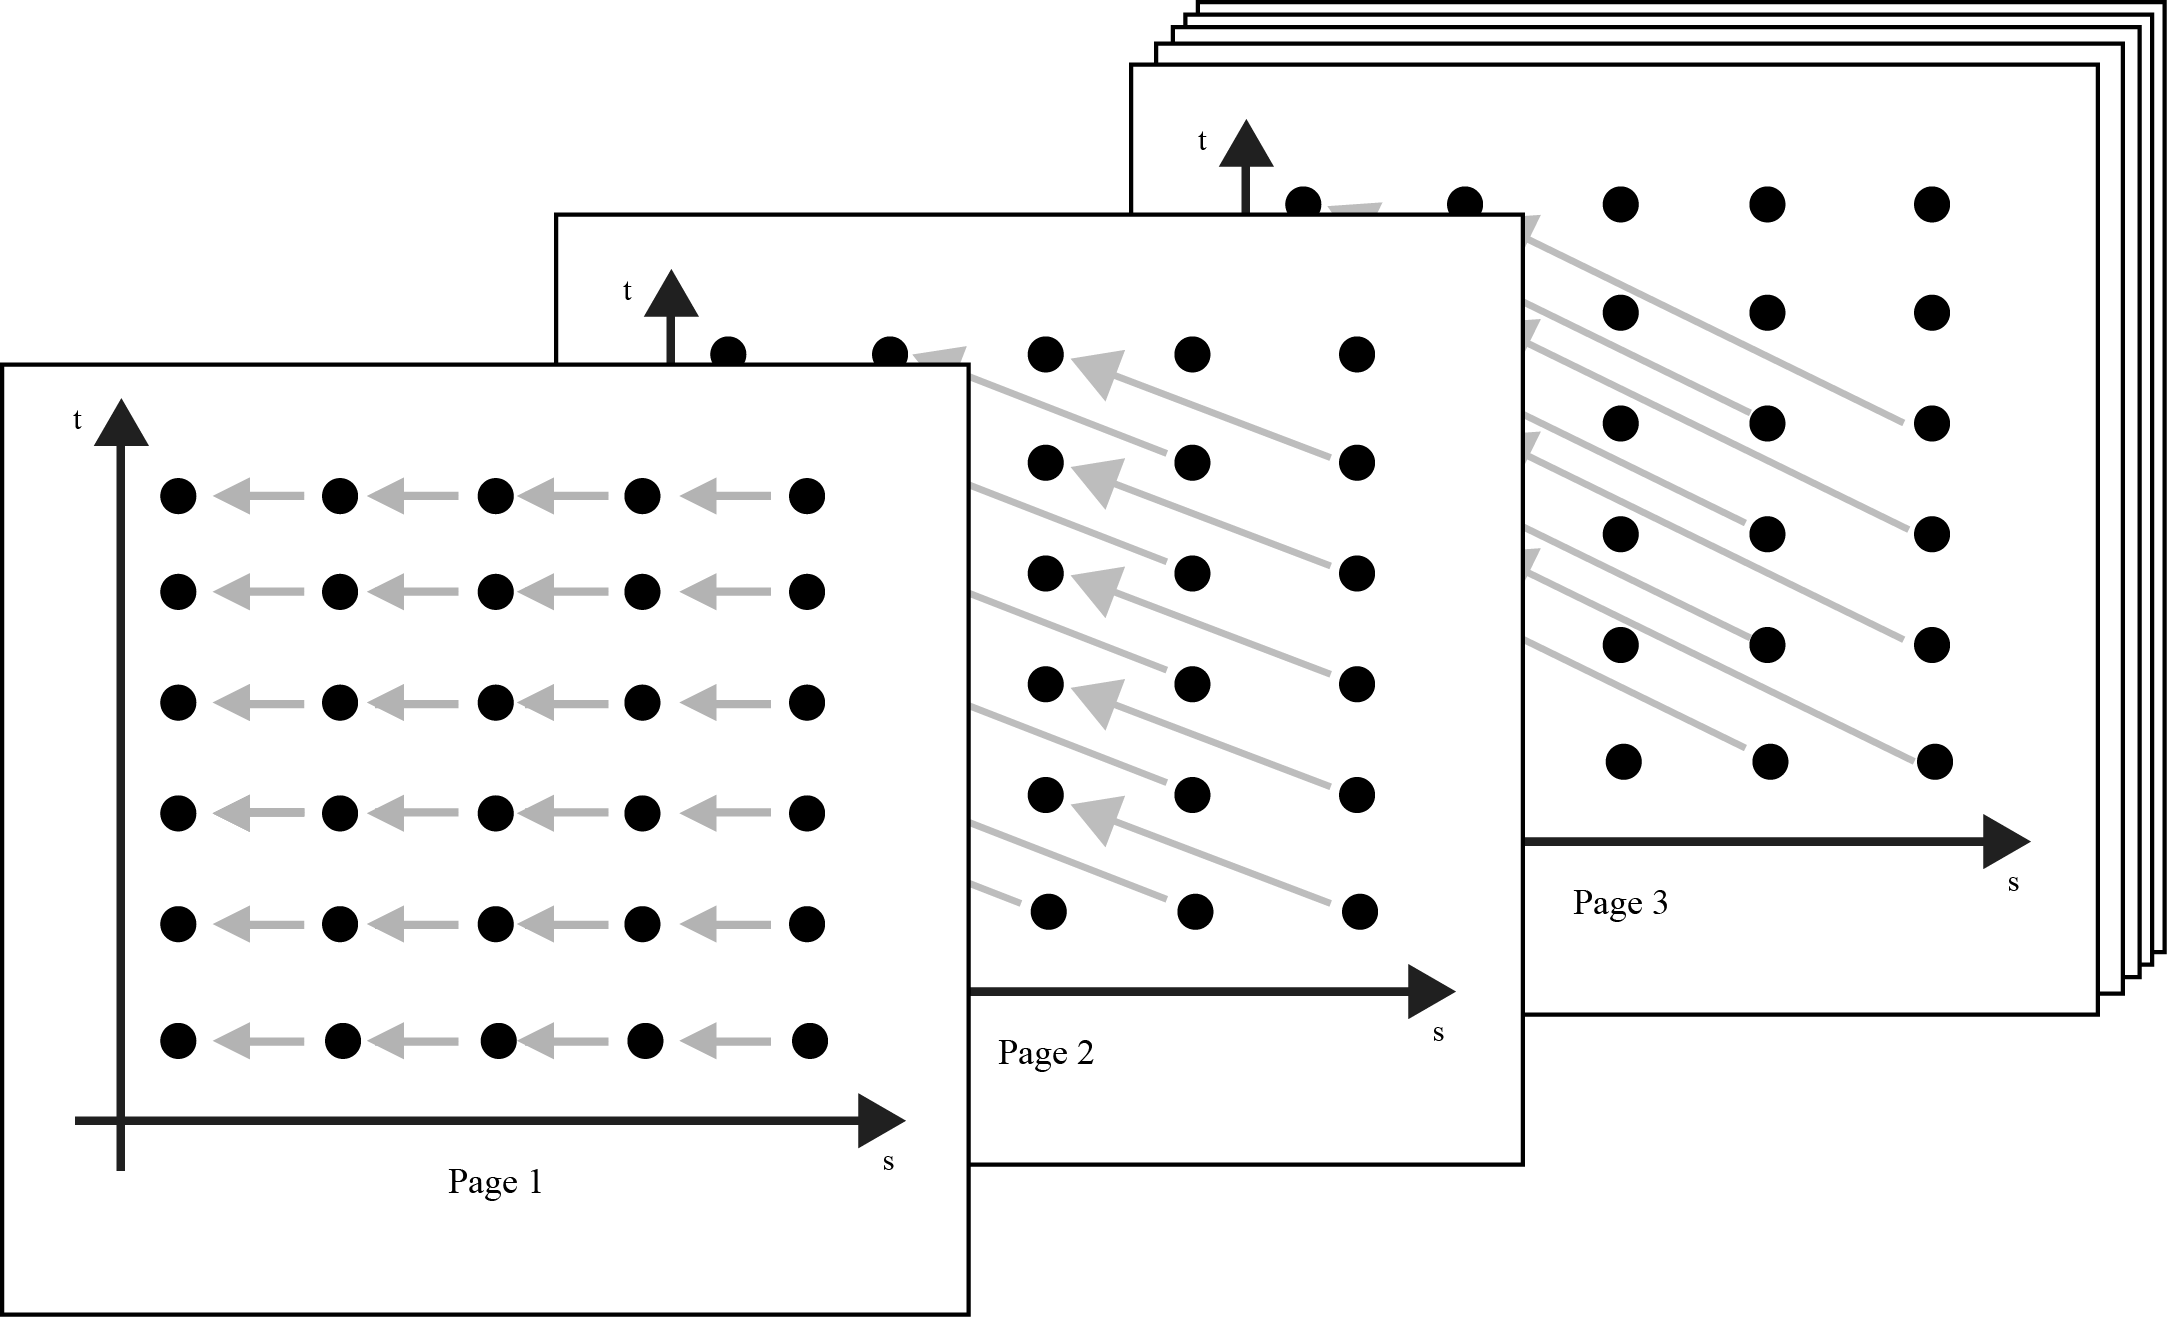
\includegraphics[width=\linewidth,height=0.5\textheight,keepaspectratio]{figures/cover.png}
  \end{center}
       \begin{minipage}{.35\linewidth}
    \begin{flushleft}
      \vspace{2em}
      {\fontsize{6pt}{2pt} \textit{Notes: These are notes live-tex'd
from a graduate course in Categorification taught by Ariki Wilbert at
the University of Georgia in Summer 2020. As such, any errors or
inaccuracies are almost certainly my own. } } \\
    \end{flushleft}
    \end{minipage}
    \hfill
    \begin{minipage}{.65\linewidth}
    \end{minipage}
  }







\begin{document}

\date{}
\maketitle
\begin{flushleft}
\textbf{D. Zack Garza} \\
\textit{University of Georgia} \\
\textit{dzackgarza@gmail.com} \\
{\tiny \textit{Last updated:} 2020-10-25 }
\end{flushleft}


\newpage
\tableofcontents

\hypertarget{monday-july-6th}{%
\section{Monday July 6th}\label{monday-july-6th}}

\hypertarget{motivation}{%
\subsection{Motivation}\label{motivation}}

We'll start with \(X\) a finite CW complex.

\begin{definition}[CW Complex]

A \textbf{CW complex} is a topological space built by inductively
attaching \(i\dash\)dimensional discs (\(i\dash\)cells)
\(\DD^i \definedas \theset{\vector x\in \RR^i \suchthat \norm{\vector x} \leq 1}\)
along their boundary
\(\bd \DD^i = S^{i-1} \definedas \theset{\vector x\in \RR^i \suchthat \norm{\vector x} = 1}\).

\end{definition}

\begin{definition}[Euler Characteristic]

Define \(\chi(X) = \sum_{i\in \ZZ} (-1)^i \abs{C_i}\) where
\(\abs{C_i}\) is the number of \(i\dash\)cells.

\end{definition}

\begin{remark}

Note that a homotopy equivalence between spaces induces an equality
between Euler characteristics.

\end{remark}

Recall that we can define the cellular chain complex
\begin{align*}
C_*^{\text{cell}}(X, \CC)\definedas \cdots \mapsvia{\del_{i+1}} C_n^{\text{cell}} (X, \CC) \mapsvia{\del_{i}} \cdots \to C_0^{\text{cell}}(X, \CC)
\end{align*}

and \(H_i(X, \CC) \definedas \ker \del_i / \im \del_{i+1}\).

\begin{exercise}[?]

\begin{align*}
\sum (-1)^i \dim H_i(X, \CC) = \chi(X)
\end{align*}

\end{exercise}

In this sense, cellular homology categorifies the Euler characteristic:
we've replaced a set of objects with a category. This is an improvement
because we may not have maps between the elements of sets, \emph{but} we
do have maps between objects in a category. We can also talk about
things such as functoriality.

\begin{example}

The euler characteristic is a weaker invariant than homology. Note that
\begin{align*}  
\chi(S^1) = 0 &\quad\text{and}\quad \chi(S^1\disjoint S^1) = 0 \\ \\ 
H_0(S^1) = \CC &\quad\text{while}\quad H_0(S^1\disjoint S^1) = \CC\oplus \CC
,\end{align*} so these aren't distinguished by euler characteristic
alone.

\end{example}

Our first goal will be to assign invariants to oriented links \(L\),
where homotopy equivalence will be replaced with isotopy. We'll assign a
Khovanov complex \(C_*(L,\CC)\), a complex of \(\ZZ\dash\)graded
\(\CC\dash\)vector spaces, along with the Jones polynomial
\(J(L) \in \ZZ[t, t\inv]\). By taking the (graded) Euler characteristic
of the chain complex, we'll recover \(J(L)\).

\hypertarget{setup}{%
\subsection{Setup}\label{setup}}

\begin{definition}[Links and Knots]

A \emph{link} \(L\) is a smooth, closed 1-dimensional embedded
submanifold of \(\RR^3\). \(L\) is a \emph{knot} if it consists of one
connected component.

\end{definition}

We have planar projections:

\begin{figure}
\centering
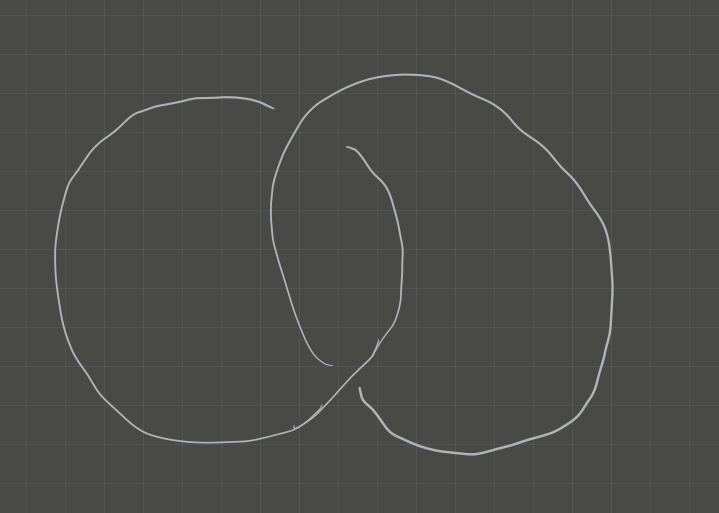
\includegraphics[width=2.60417in,height=\textheight]{figures/image_2020-07-06-11-30-13.png}
\caption{Planar projection of the Hopf link}
\end{figure}

Under this correspondence, isotopy of knots will correspond to planar
isotopy of the diagrams and the following 3 Reidemeister moves:

\begin{definition}[Reidemeister Moves]

There are three planar moves that preserve the isotopy class of a planar
projection of a knot:

\begin{figure}
\centering
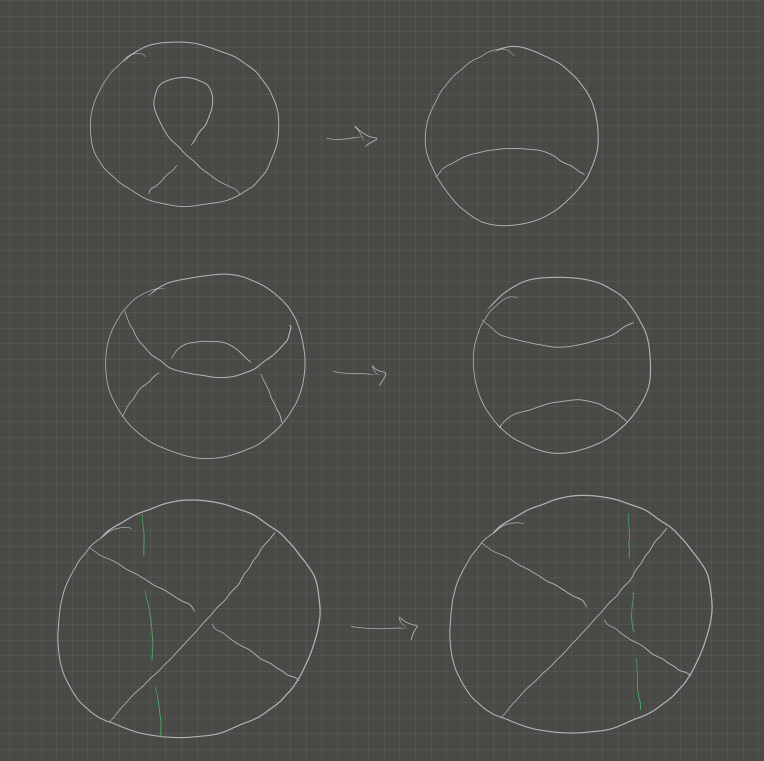
\includegraphics[width=3.125in,height=\textheight]{figures/image_2020-07-06-11-31-38.png}
\caption{Reidemeister Moves}
\end{figure}

\end{definition}

\begin{example}

How to change knot diagrams using Reidemeister moves:

\begin{figure}
\centering
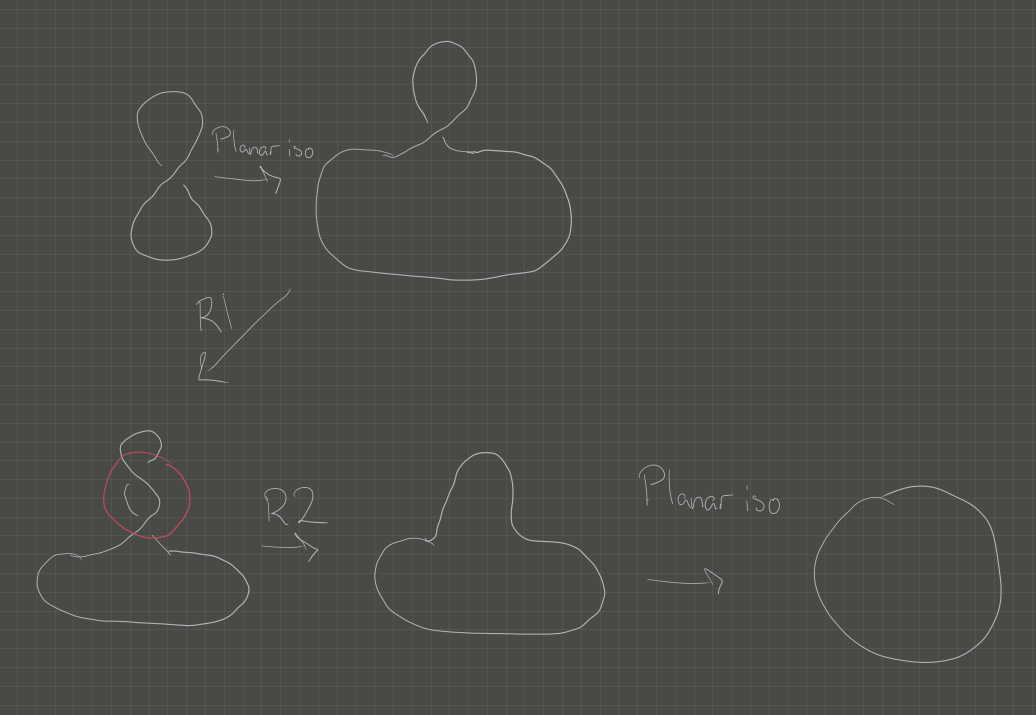
\includegraphics[width=4.16667in,height=\textheight]{figures/image_2020-07-06-11-35-44.png}
\caption{Changing knot diagrams using Reidemeister moves.}
\end{figure}

\end{example}

We now want to take an oriented, planar link diagram \(D\) and associate
to it a polynomial \(J(D)\). We start by defining the Kauffman bracket

\begin{definition}[Kauffman Bracket]

Let \(D_f\) be \(D\) with the orientation forgotten, then
\(\gens{D_f} \in \ZZ[v, v\inv]\) is defined recursively by

\begin{figure}
\centering
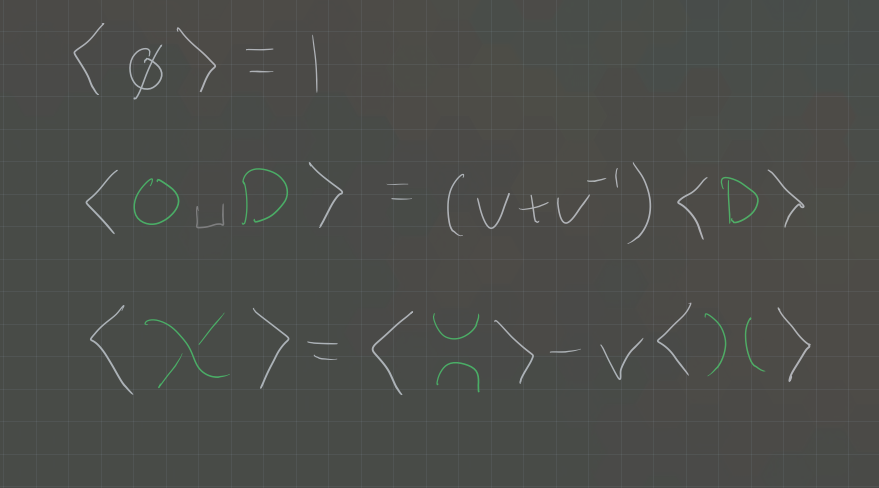
\includegraphics[width=4.16667in,height=\textheight]{figures/image_2020-07-06-11-40-29.png}
\caption{Recursive definition of Kaufman bracket}
\end{figure}

In the last case, the first term is a ``0-resolution/0-smoothing'' and
the second is a ``1-resolution/1-smoothing''.

\end{definition}

\begin{definition}[Positive and Negative Crossings]

We have a notion of positive/negative crossings:

\begin{figure}
\centering
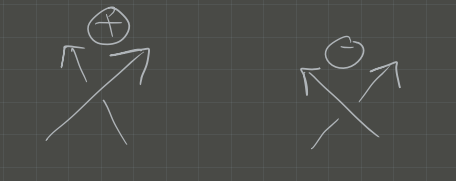
\includegraphics[width=3.125in,height=\textheight]{figures/image_2020-07-06-11-44-50.png}
\caption{Positive and negative crossings.}
\end{figure}

\end{definition}

\begin{definition}[The Jones Polynomial]

We set
\begin{align*}
J(D) = (-1)^{n_-} v^{n^+ - 2n_-} \gens{D_f}
.\end{align*}

\end{definition}

\begin{example}

\hfill

\begin{enumerate}
\def\labelenumi{\arabic{enumi}.}
\item
  \(J(S^1) = v + v\inv\)
\item
  \(J(?) = (-1) v^{-2} \qty{ -v^2 (v+v\inv)} = v+v\inv\).
\item
  \(J(?) = v^{-6} + v^{-4} + v^{-2} + 1\)
\end{enumerate}

\begin{figure}
\centering
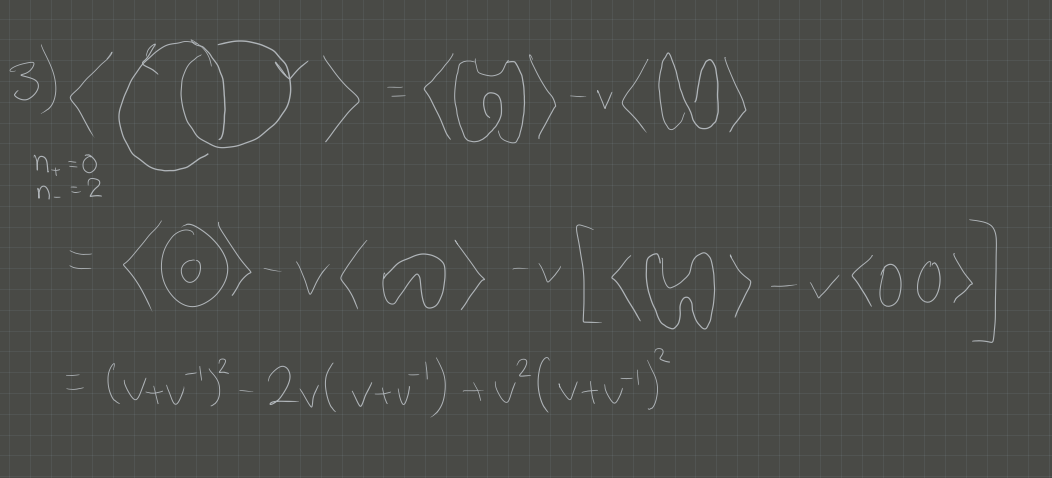
\includegraphics{figures/image_2020-07-06-11-50-40.png}
\caption{Bracket of the Hopf link.}
\end{figure}

\end{example}

\begin{proposition}[Invariance under Reidemeister moves]

The Jones polynomial is invariant under move \(R1\).

\end{proposition}

\begin{proof}

Can be checked in diagrams:

\begin{figure}
\centering
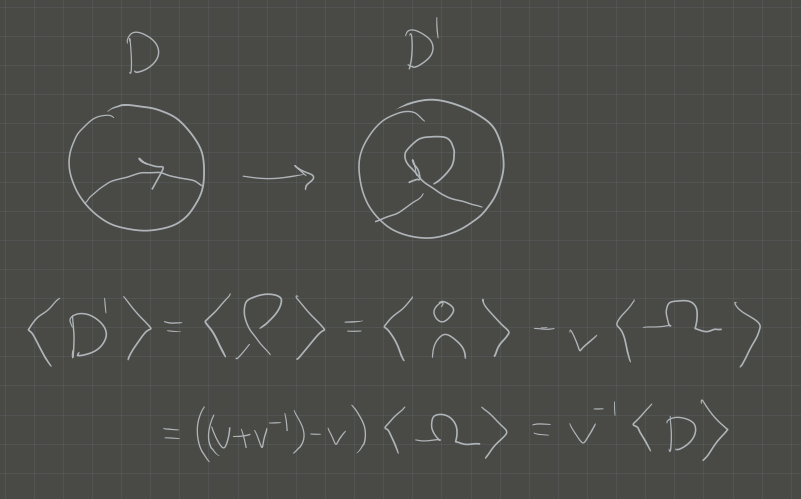
\includegraphics[width=4.6875in,height=\textheight]{figures/image_2020-07-06-11-54-27.png}
\caption{\(J(D') = J(D)\)}
\end{figure}

\end{proof}

\begin{remark}

You can now check that
\begin{align*}
J(D') = (-1)^{n_-(D)} v^{n_+(D) + 1} - 2n_-
.\end{align*}

\end{remark}

\begin{exercise}[?]

Check invariance under R2, R3.

\end{exercise}

\hypertarget{tuesday-july-7th}{%
\section{Tuesday July 7th}\label{tuesday-july-7th}}

Recall that we had recursive rules for computing the Kausffman bracket,
and a normalization factor for the Jones polynomial that made it into an
invariant. We'd like a closed formula for these.

We do this by ordering the crossings of the unoriented link
\(1, \cdots, n\), then there is a correspondence
\begin{align*}
\theset{0, 1}^n &\iff \text{Complete resolutions} \\
(\alpha_1, \cdots, \alpha_n) &\iff \alpha_i \text{ resolves the $i$th crossing}
.\end{align*}

\begin{example}

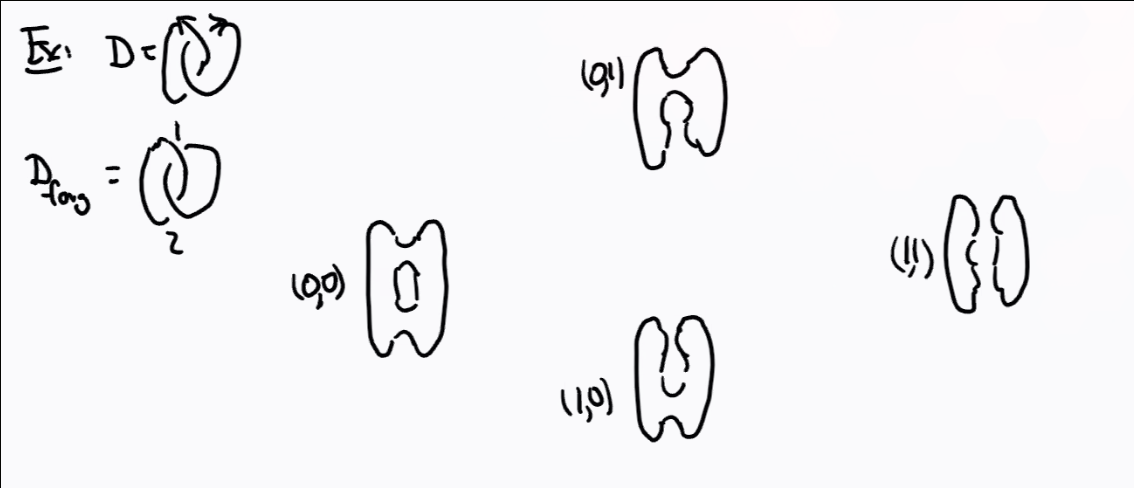
\includegraphics{figures/image_2020-07-07-11-07-33.png}

\end{example}

\begin{claim}

\begin{align*}
\gens{D} = \sum_{\alpha \in \theset{0, 1}^n} (-1)^{\abs \alpha}  v^{\abs \alpha} (v+v\inv)^{c_\alpha(D)}
,\end{align*}

where \(\abs \alpha\) is the number of 1-resolutions and \(c_\alpha\) is
the number of circles in the resolution corresponding to \(\alpha\).

\end{claim}

\begin{proof}

Idea: look at resolving the \(n\)th crossing locally and apply the
recursive relation. Then rewrite the sum by appending \(\alpha_n = 0\)
and \(\alpha_n = 1\) respectively. Note that we can rewrite the sum as
\begin{align*}
\sum_{r=0}^n (-1)^r \sum_{\abs \alpha = r} v^r (v+v\inv)^{c_\alpha(D)}
.\end{align*}

This amounts to summing over the ``columns'' in the previous diagram:

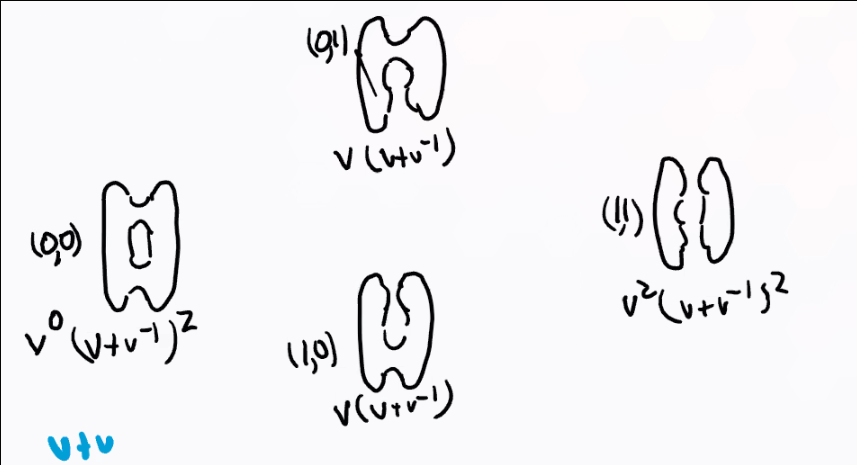
\includegraphics{figures/image_2020-07-07-11-22-49.png}

Here this yields
\begin{align*}
(v+v\inv)^2 + (-1)2v(v+v\inv) + v^2 (v+v\inv)^2
.\end{align*}

\end{proof}

Note that this formula starts to resemble an Euler characteristic!

\begin{remark}

\emph{Problem}: The coefficient
\begin{align*}
\sum v^r(v+v\inv)^{c_\alpha(D)} \in \ZZ^{\geq 0}[v, v\inv]
\end{align*} is a Laurent polynomial instead of a natural number, so
this can't immediately be interpreted as a dimension of a vector space.

\emph{Solution}: Replace finite-dimensional \(\CC\dash\)vector spaces by
\(\ZZ\dash\)graded vector spaces. The category consists of objects given
by \(V = \bigoplus_{i\in \ZZ} V_i\) and linear maps \(f:V\to W\) such
that \(f(V_i) \subseteq W_i\) for all \(i\).

\end{remark}

We previously had vector spaces categorifying the natural numbers by
taking the dimension, so for graded vector spaces, we take the
\textbf{graded dimension}:

\begin{definition}[Graded Dimension]

\begin{align*}
\grdim \bigoplus_{i\in\ZZ}V_i = \sum_{i\in \ZZ}\qty{\dim V_i}v^i \in \ZZ^{\geq 0}[v, v\inv]
.\end{align*}

\end{definition}

\textbf{Goal}: We want to associate to an oriented link diagram \(D\) a
cochain complex of finite-dimensional graded \(\CC\dash\)vector spaces
\(C_i(D) \mapsvia{\bd} C_{i+1}(D) \to \cdots\). Since each chain space
decomposes, the differential does as well, and we get a large collection
of chain complexes

\begin{center}\includesvg[width=0.7\linewidth]{889e18b18376b9cf8c5bd5199f934098b01a0edd}\end{center}

This yields two gradings: the first is homological, the second is
``internal''.

\begin{remark}

We want the following:

\begin{enumerate}
\def\labelenumi{\arabic{enumi}.}
\item
  If \(D, D'\) are related by a finite sequence of Reidemeister moves,
  then
  \begin{align*}
  H_{i, j}(C_{\wait, \wait}(D)) = H_{i, j}(C_{\wait, \wait}(D')) = \ker \bd_{i, j} / \im \bd_{i-1, j} \text{ for all }i, j.
  \end{align*}
\item
  Additionally,
  \begin{align*}
  J(D) = \chi_{\gr}(C_{*, *}(D)) = \sum_{i\in \ZZ} (-1)^i \grdim \qty{ C_{*, *}(D) }
  \end{align*}
\end{enumerate}

Note that you can also take the dimension of the homology instead, and
at the end of the day this yields
\(\sum_{i, j\in \ZZ} (-1)^i v^j \dim(H_{i, j})\).

\end{remark}

\begin{definition}[Homogeneous elements]

For \(A = \bigoplus A_i, B = \bigoplus B_i\), \(a\in A\) is called
\emph{homogeneous} of degree \(k\) if \(a\in A_k\), i.e.~it is a sum of
basis elements from only the \(k\)th graded piece. In this case we say
\(\abs a = k\).

\end{definition}

\begin{proposition}[Bases for various combinations of graded spaces]

We can union bases over all graded pieces to get a basis for the entire
space.

For direct sums \(A\oplus B\), a basis is given by \((\alpha_i, 0)\) and
\((0, \beta_j)\). We put \(\alpha_i\) in degree \(\abs{\alpha_i}\), in
which case
\begin{align*}
\grdim(A\oplus B) 
&= \sum_{k\in \ZZ} \dim(\qty{A\oplus B}_k) v^k \\
&= \sum_k \dim A_k v^k + \sum \dim B_k v^k \\
&= \grdim(A) + \grdim(B)
,\end{align*} so taking direct sums commutes with taking graded
dimensions.

Similarly for tensor products \(A\tensor_\CC B\), we get a basis
\(\alpha_i \tensor \beta_j\) placed in degree
\(\abs{\alpha_i} + \abs{\beta_j}\).

\end{proposition}

\begin{exercise}[?]

Show that
\begin{align*}
\grdim(A\tensor_\CC B) = \grdim(A) \cdot \grdim(B)
.\end{align*}

\end{exercise}

We also have degree shifts by \(i\) for any \(i\), denote \(A(i)\),
where \(A_j \mapsto A_{j+i}\) for every \(j\). Thus the \(k\)th graded
piece is given by \((A(i))_k = A_{k-i}\), thus
\begin{align*}
\grdim(A(i)) = v^i \grdim(A)
\end{align*}

\begin{example}[Important]

\begin{align*}  
H^*(S^2; \CC)
=
\begin{cases}
\CC & * = 0, 2 \\
0 & \text{else}.
\end{cases}
\end{align*}

Let \(A\definedas H^*(S^2; \CC)(-1)\), which now has \(\CC\) in degrees
\(\pm 1\), and \(\grdim A = v + v\inv\).

Note that

\begin{itemize}
\tightlist
\item
  \((v+v\inv)^2\) corresponds to \(A^{\tensor 2}\).
\item
  \(2v(v+v\inv)\) corresponds to \(A(1)^{\oplus 2}\).
\item
  \(v^2(v+v\inv)\) corresponds to \(A^{\tensor 2}(2)\).
\end{itemize}

So we can assemble these into a chain complex and take the Euler
characteristic in order to recover the Kauffman bracket in the earlier
example.

\end{example}

\begin{theorem}[?]

There exists a unique isotopy invariant of oriented links in \(\RR^3\)
called \(P(D) \in \CC(a, v)\), a rational function in two variables, the
HOMFLY-PT polynomial. It satisfies

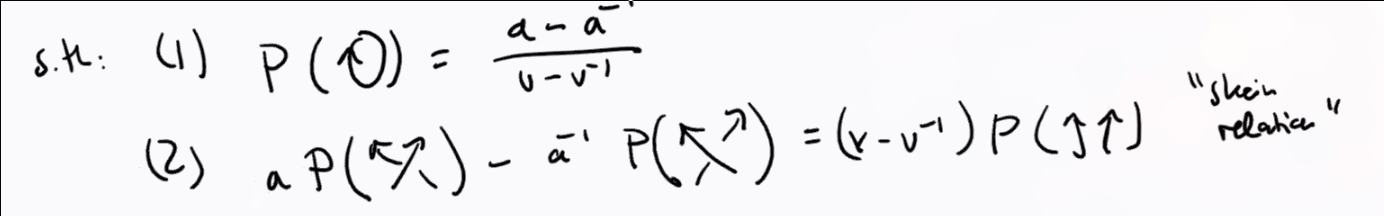
\includegraphics{figures/image_2020-07-07-11-56-40.png}

\end{theorem}

\begin{example}[The Hopf Link]

Yields
\begin{align*}
P(D) = -a(aia\inv) + a^2 \qty{a-a\inv \over v-v\inv}^2
.\end{align*}

\end{example}

\hypertarget{wednesday-july-8th}{%
\section{Wednesday July 8th}\label{wednesday-july-8th}}

Recall that we assigned a chain complex of graded vector spaces to
links, where the chains where various tensor powers and shifts of
\(\mca \definedas H^*(S^2; \CC)(-1)\). We can consider the diagonal
embedding
\begin{align*}
S^s \mapsvia{\Delta} S^2 \cross S^2
\end{align*}

which induces maps on both cohomology and homology, and applying the
Kunneth formula and the Poincare isomorphism, we get maps
\begin{align*}
m:      H^*(S^2)^{\tensor 2} &\to H^*(S^2) \\
\delta: H^*(S^2) &\to H^*(S^2)^{\tensor 2}
.\end{align*}

We thus get maps
\begin{align*}
m:        \CC[x]/(x^2) \tensor \CC[x]/(x^2) &\to \CC[x]/(x^2) \\
\delta:   \CC[x]/(x^2) &\to \CC[x]/(x^2) \tensor \CC[x]/(x^2)
.\end{align*}

See course notes for how to construct differentials out of these,
categorifying the bracket, and how to correct with shifts to categorify
the Jones polynomial.

\hypertarget{lecture-3}{%
\subsection{Lecture 3}\label{lecture-3}}

\begin{definition}[Geometric Braids]

For \(n\geq 1\), the geometric braid \(b\) on \(n\) strands is a
topological subspace of \(\RR^2 \cross [0, 1]\) such that

\begin{enumerate}
\def\labelenumi{\alph{enumi}.}
\tightlist
\item
  \(b \cong \disjoint_{i=1}^n [0, 1]\) is a homeomorphism
\item
  We have
  \begin{align*}
    b\intersect (\RR^2 \cross \theset{0}) &= \theset{(1,0,0), \cdots, (n,0,0)} \\
    b\intersect (\RR^2 \cross \theset{1}) &= \theset{(1,0,1), \cdots, (n,0,1)}
    .\end{align*}
\item
  The projection \(\RR^2 \cross [0, 1] \mapsvia{\pr_2}\) maps each
  strand homeomorphically onto \([0, 1]\).
\end{enumerate}

\end{definition}

\begin{remark}

Braids can be moved via isotopy, and part (c) prevents the following
situation:

\begin{figure}
\centering
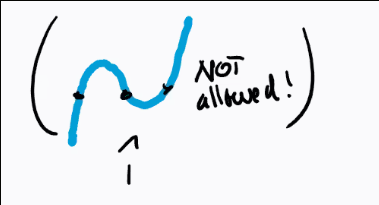
\includegraphics[width=2.60417in,height=\textheight]{figures/image_2020-07-08-11-38-02.png}
\caption{Situation to rule out.}
\end{figure}

\end{remark}

There is a purely combinatorial description, namely braid diagrams.
Isotopies on the geometric side will correspond to planar isotopies and
Reidemeister moves R2 and R3 (since R1 is ruled out).

\begin{figure}
\centering
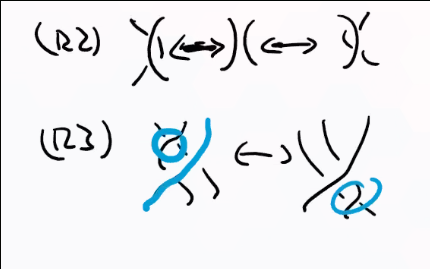
\includegraphics[width=2.60417in,height=\textheight]{figures/image_2020-07-08-11-42-13.png}
\caption{Moves 2 and 3.}
\end{figure}

\begin{theorem}[?]

Two braids are isotopic iff their diagrams are related by planar isotopy
and a finite sequence of Reidemeister moves.

\end{theorem}

\begin{definition}[The Braid Monoid]

Define \(B_n\) to be the set of braid diagrams on \(n\) strands up to
isotopy and Reidemeister moves, then there is a multiplication given by
stacking braid diagrams. This is associative with identity, so we obtain
a monoid:

\begin{figure}
\centering
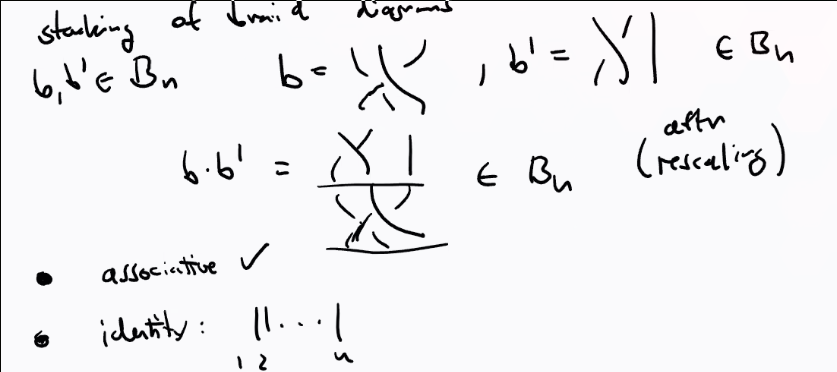
\includegraphics[width=6.77083in,height=\textheight]{figures/image_2020-07-08-11-45-36.png}
\caption{Braid monoid.}
\end{figure}

\end{definition}

\begin{definition}[Elementary braids]

We define elementary braids:

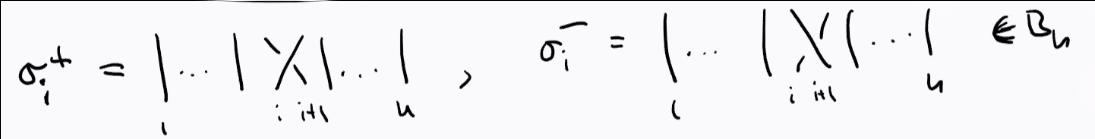
\includegraphics{figures/image_2020-07-08-11-46-13.png}

\end{definition}

\begin{remark}

\hfill

\begin{itemize}
\item
  \(\theset{\sigma_i^\pm}_{i=1}^{n-1}\) generates \(B_n\) as a monoid,
  so \(\beta \in B_n\) implies
  \begin{align*}
  \beta = \prod_{k=1}^n \sigma_{i_k}^{\eps_k} \text{ where } i_k \in \theset{1, \cdots, n-1} \text{ and }\eps_j \in \theset{\pm 1}
  .\end{align*}
\item
  \(\sigma_i^+ \sigma_i^- = \sigma_i^- \sigma_i^+ = 1\) for all \(i\),
  thus every braid \(b\) has a two-sided inverse given by reversing the
  \(\sigma_{i_k}\)s and swapping \(\pm\), so \(B_n\) is a group.
\end{itemize}

We can describe this group completely algebraically as
\(B_n^{\text{Artin}}\), the group generated by
\(\theset{\sigma_i}_{i=1}^{n-1}\) with relations
\begin{align*}  
\sigma_i \sigma_j &= \sigma_j \sigma_i && \text{for } \abs{i-j} \geq 2 \\ 
\sigma_i \sigma_{i+1} \sigma_i &= \sigma_{i+1} \sigma_i \sigma_{i+1} &&  \text{for } i\in \theset{1, \cdots, n-2}
.\end{align*}

\end{remark}

\begin{proposition}[?]

There is an isomorphism
\begin{align*}
B_n^{\text{Artin}} &\mapsvia{\cong} B_n \\
\sigma_i &\mapsto \sigma_i^+ \\
\sigma_i\inv &\mapsto \sigma_i^-
.\end{align*}

\end{proposition}

\begin{proof}

\hfill

\textbf{Well defined}: Need to check that the map preserves the
relations, this is a consequence of changing height of crossings by
planar isotopy:

\begin{figure}
\centering
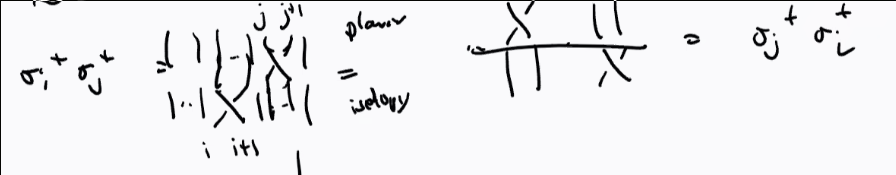
\includegraphics{figures/image_2020-07-08-11-56-18.png}
\caption{Changing heights of crossings.}
\end{figure}

\begin{figure}
\centering
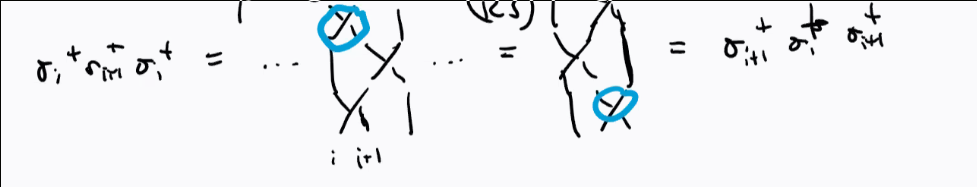
\includegraphics{figures/image_2020-07-08-11-57-06.png}
\caption{Changing heights of crossings.}
\end{figure}

\begin{itemize}
\item
  Surjectivity: clear by definition of map.
\item
  Injectivity: omitted.
\end{itemize}

\end{proof}

\begin{remark}

Importantly, we have a way of going from braids to knots and links. Let
\(D^{\text{or}}\) be the set of oriented planar link diagrams, then
define a map
\begin{align*}
B_n &\to D^{\text{or}} \\
b &\mapsto \hat b
\end{align*}

where \(\hat b\) is given by ``closing'' the braid:

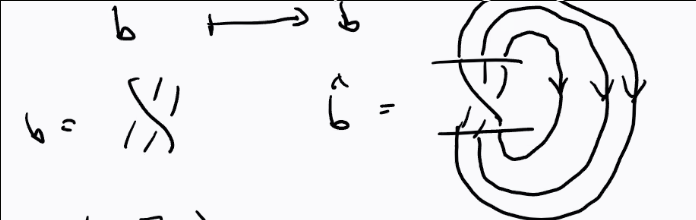
\includegraphics{figures/image_2020-07-08-12-00-35.png}

\end{remark}

\begin{theorem}[?]

Every oriented link in \(\RR^3\) is isotopic to a closed braid.

\end{theorem}

\begin{remark}

In fact, there is a map
\begin{align*}
\disjoint_{n\geq 1} &\surjects D^{\text{or}} /\sim \\
b & \mapsto \hat b
\end{align*}

where the RHS is the equivalence relation generated by planar isotopy
and Reidemeister moves. This is not injective, since many braids can map
onto the unknot.

\end{remark}

\hypertarget{thursday-july-9th}{%
\section{Thursday July 9th}\label{thursday-july-9th}}

Problem: the map sending links to the Artin braid group is surjective
but not injective, so we need to mod out by some form of equivalence in
the domain.

We have a directed system of inclusions \(B_n \injects B_{n+1}\), so we
can consider the group \(\disjoint_{n\geq 1} B_n\). The equivalence
relation we'll take is \emph{Markov equivalence} \(\sim_M\):

\begin{theorem}[?]

\(b \sim_M b' \iff ?\)

\end{theorem}

\begin{proof}

For the reverse direction

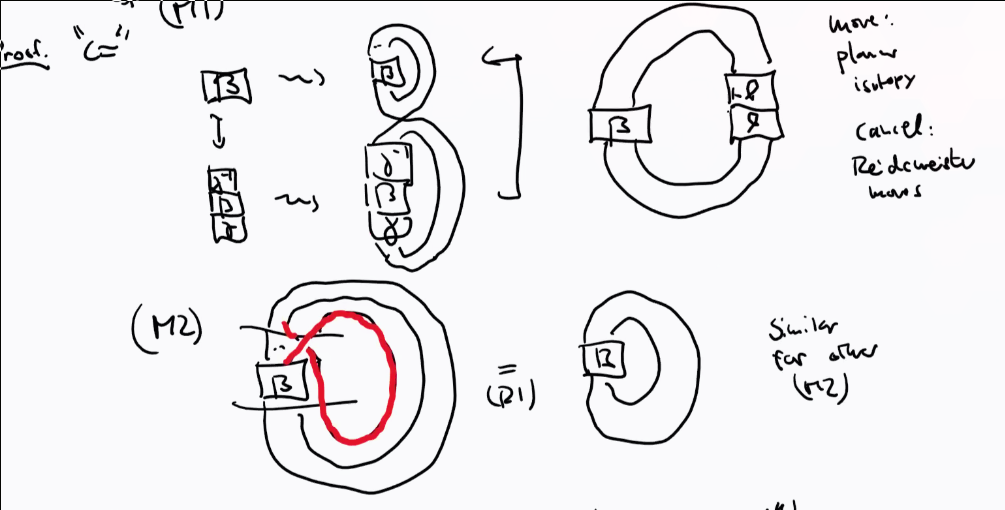
\includegraphics{figures/image_2020-07-09-11-17-40.png}

For the forward direction, see Kassel-Tuvaev's ``Braid Groups'' for a
full rigorous proof.

\end{proof}

\begin{definition}[?]

For any set \(E\), a \emph{Markov function} is a family of maps
\(\theset{f_n: B_n \to E}_{n\geq 1}\) such that

\begin{enumerate}
\def\labelenumi{\arabic{enumi}.}
\item
  \(f_n(\alpha \beta) = f_n(\beta\alpha)\) for all
  \(\alpha, \beta\in B_n\)
\item
  \(f_{n+1}(i_n(\beta)\sigma_n\inv) = f_n(\beta) = f_{n+1}(i_n(\beta) \sigma_n)\)
  for all \(n\geq, \beta \in B_n\).
\end{enumerate}

\end{definition}

\emph{Question}: where does the skein relation come from?

Take \(\FF_q\) a finite field of size \(q\) and set
\(G = \Gl(n, \FF_q)\). Define \(C(G) = \theset{G\to \CC}\) which is a
\(\CC\dash\)vector space with an associative multiplication given by
\begin{align*}
(f\ast f')(g) \da \sum_{n\in G} f(n) f'(n\inv g)
\end{align*}

Define
\begin{align*}
C\qty{\dcoset{B}{G}{B}} = \theset{f: G\to \CC \suchthat f(bg) = f(g) = f(gb)}
\end{align*} the set of bi-invariant functions. This is closed under
\(\ast\) with a unit defined by setting
\begin{align*}  
\delta_g(h) &= \indic{h=g} \\
\delta_0 &= {1\over \abs B} \sum_{g\in B} \delta_g
.\end{align*}

There is an augmentation map
\begin{align*}  
\eps: \qty{\dcoset B G B} &\to \CC \\
f &\mapsto  \sum_{g\in G} f(g) \in \CC
.\end{align*} which is a \(\CC\dash\)algebra morphism. Can we write down
a basis?

Recall that the symmetric group is generated by adjacent transpositions,
say \(s_1, \cdots, s_{n-1}\), so we can write
\begin{align*}
S_n \cong \gens{\bar s_1, \cdots, \bar s_{n-1} \suchthat \bar s_i^2 = 1, \bar s_i \bar s_j = \bar s_j \bar s_i, \bar s_i \bar s_{i+1} \bar s_i = \bar s_{i+1} \bar s_i \bar s_{i+1} }
.\end{align*}

\begin{quote}
Need to check that elements in \(S_n\) satisfy these relations, check
cardinality, etc.
\end{quote}

For any \(w\in S_n\), we can consider its length \(\ell(w)\) defined as
the smallest number of adjacent transpositions need to write \(w\) as a
product of adjacent transpositions. We define the \emph{Bruhat cell}
\(B w B \definedas \theset{bwb\inv \suchthat b, b' \in B}\) where \(B\)
is a permutation matrix for \(w\).

\begin{figure}
\centering
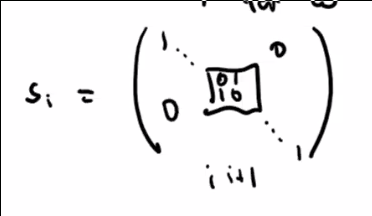
\includegraphics{figures/image_2020-07-09-11-37-26.png}
\caption{Example of a permutation matrix for \(s_i\)}
\end{figure}

\begin{exercise}[?]

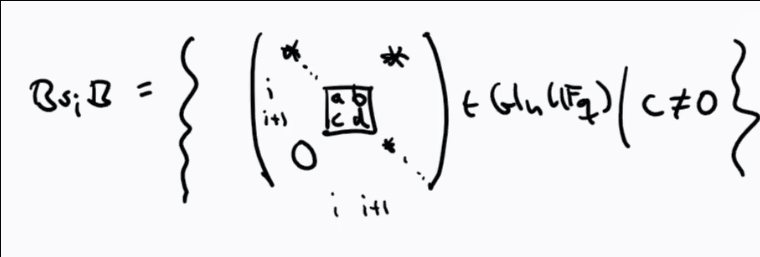
\includegraphics{figures/image_2020-07-09-11-38-04.png}

\end{exercise}

\begin{proposition}[?]

The functions
\begin{align*}
\delta_w: G &\to \CC \\
\delta_w(g) &= {1\over \abs B}\indic{g\in BwB}
\end{align*} as \(w\) ranges over \(S_n\) form a basis for
\(\qty{\dcoset B G B}\).

\end{proposition}

\begin{proof}

Use the Bruhat decomposition \(G = \disjoint_{w\in S_n} BwB\).

\end{proof}

\hypertarget{multiplicative-structure}{%
\subsection{Multiplicative Structure}\label{multiplicative-structure}}

There is a multiplicative structure, since
\begin{align*}
(\delta_{s_i} \ast \delta_{s_i})(g) 
&\definedas \sum_{h\in G} \delta_{s_i}(h) \delta_{s_i}(h\inv g) \\
&= \sum_{h\in Gs_i B} {1\over \abs B} \delta_{s_i} (h\inv g) \\ \\
&= \sum_{\substack{ h\in S }} 
{1\over \abs{B}^2}
&& S = \ts{h\in B_{s_i} B \st h^{-1} g \in B_{s_i} B} \\
&= {\abs{Bs_i B \intersect gBs_i B} \over \abs{B}^2}
.\end{align*}

To express this in terms of our basis, check where
\(B_si B \intersect g B s_i B \neq \emptyset\). If \(h\) is in this
intersection, then \(h = bs_i b = gb'' s_i b'''\), so
\begin{align*}
g = b s_i b' (b''')\inv s_i (b'')\inv \in Bs_i Bs_i B \subset P_i
\end{align*} where \(P_i\) is a parabolic subgroup of \(G\) defined by

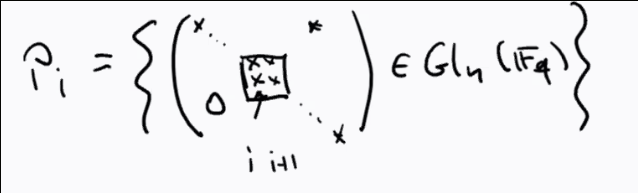
\includegraphics{figures/image_2020-07-09-11-47-18.png}

We can identify \(P_i = Bs_i B \union B\) (i.e.~add in upper triangular
matrices). We can thus write
\(\delta_{s_i} \ast \delta_{s_i} = \alpha \delta_{s_i} + \beta \delta_0\)
where \(\delta_0 = \delta_e\) and \(\alpha, \beta \in \CC\).

Let \(\bbone\) be the identity matrix, then

\begin{align*} 
{\abs{B s_i B} \over \abs{B}^2} 
= (\delta_{s_i} \ast \delta_{s_i}) (\bbone) 
= \alpha \delta_{s_i} + \beta \delta_0(\bbone)
.\end{align*}

where the first term is in \(B\) and thus equals zero, and the second
term equals \(1\over \abs B\), so this equals \(\beta{1\over \abs{B}}\),
thus \(\beta = {\abs{Bs_i B} \over \abs{B} }\). Similarly, we get
\(\alpha = {\abs{Bs_i B} \over \abs B} - 1\).

A counting argument shows
\begin{align*}
\abs{B} = (q-1)^n q q^2 \cdots q^{n-1} = (1-1)^n q^{n(n-1) \over 2}
.\end{align*}

Similarly
\begin{align*}
\abs{Bs_i B} = (q-1)^n q^{{n(n-1) \over 2} + 1}
\implies 
{\abs{Bs_i B} \over \abs B} = 1
.\end{align*} Thus
\begin{align*}
(\delta_{s_i} \ast \delta_{s_i}) 
= (q-1) \delta_{s_i} + q\delta_0
.\end{align*}

In particular, \(\delta_{s_i}\) is a unique with inverse
\(q\inv \delta_{s_i} - (1-q\inv) \delta_0\).

\begin{claim}

More generally, for \(s_i \in S_n, w\in S_n\) with
\(\ell(s_i w) > \ell(w)\), we have
\(\delta_{s_i} \ast \delta_w = \delta_{s_i w}\).

\end{claim}

\begin{proof}

Omitted, see Bump ``Hecke Algebras''.

\end{proof}

Upshot: we have a group morphism
\begin{align*}
\phi: B_n &\to C\qty{\dcoset B G B}\units \\
\sigma_i &\mapsto \delta_{s_i}
.\end{align*}

Need to check that this is well-defined using the braid relations, comes
from
\begin{align*}
\delta_{s_i} \ast \delta_{s_j} = \delta_{s_i s_j} = \delta_{s_j s_i} = \delta_{s_j} \ast \delta_{s_i}
\end{align*}

\hypertarget{friday-july-10th}{%
\section{Friday July 10th}\label{friday-july-10th}}

\hypertarget{the-iwahori-hecke-algebra}{%
\subsection{The Iwahori-Hecke Algebra}\label{the-iwahori-hecke-algebra}}

\begin{definition}[Iwahori-Hecke Algebra]

For \(n\geq 1\) and \(R\) a commutative ring with \(q,z \in R\units\),
define the \emph{Iwahori-Hecke algebra} \(H_n^R(q, z)\) is the
associative unital \(R\dash\)algebra
\begin{align*}
\gens{T_i \suchthat R} \text{where the relations $R$ are defined by } \\
T_i T_j &= T_j T_i && \abs{i - j} \geq 2 \\
T_i T_{i+1} T_i &= T_{i+1} T_i T_{i+1} \\
T_i^2 &= zT_i q1
\end{align*} where \(1\) is the unit of the algebra. The first relation
is the \emph{braid relation}, the other two are \emph{quadratic} or
\emph{skein} relations.

\end{definition}

\begin{theorem}[Basis of the Hecke Algebra]

\hfill

\begin{enumerate}
\def\labelenumi{\arabic{enumi}.}
\tightlist
\item
  For all \(w \in S_n\), there exists a unique \(T_w\in H_n^R(q, z)\)
  such that whenever \(w = \prod s_{i_k}\) is a minimal expression as a
  product of simply transpositions, then \(T_w = \prod T_{i_k}\).
\item
  The set \(\theset {T_w \suchthat w\in S_n}\) is an \(R\dash\)module
  basis of \(H_n^R(q, z)\) (the standard basis).
\end{enumerate}

\end{theorem}

\begin{remark}

\hfill

\begin{enumerate}
\def\labelenumi{\arabic{enumi}.}
\item
  \(H_n^R(q, z)\) is a two-parameter generalization of
  \(C(\dcoset B G B)\), and in fact there is an \(R\dash\)algebra
  isomorphism
  \begin{align*}
  H_n^\CC(q, q-1) &\cong C(\dcoset B G B)\\
  T_w &\mapsto \delta_w
  .\end{align*}
\item
  There is an \(R\dash\)algebra isomorphism
  \(H_n^R(1, 0) \cong R[S_n]\), so we interpret this as a deformation of
  the group algebra \(R[S_n]\).
\item
  There is an \(R\dash\)algebra isomorphism
\end{enumerate}

\begin{align*}
  H_n^R(q, z) \cong H_n^R(q, z) \cong R[B_n] / \gens{T_i^2 - zT_i - q\cdot 1}
  \end{align*} as a quotient of the group algebra on the braid group.

There is also an \(R\dash\)algebra morphism
\begin{align*}
\iota_n: H_n^R(q, z) &\to H_{n+1}^R(q, z) \\
T_i &\mapsto T_i
.\end{align*}

\end{remark}

\begin{theorem}[?]

There exists a unique collection of \(R\dash\)linear maps for
\(n\geq 1\):
\begin{align*}
\tr_n: H_n^R(q, z) &\to R
.\end{align*}

This is uniquely determined by the properties
\begin{align*}
\tr_n(ab) &= \tr_n(ba) 
&& \forall a,b\in H_n^R(q ,z) \\
\tr_{n+1}(\iota(a) T_n) &= \tr_n(a) = \tr_{n+1} (\iota(a) T_n\inv) 
&&\forall a\in H_n^R(q, z) \\
\tr_{n+1}(\iota(a)) &= {1 - q \over z} \tr_n(a) 
&&\forall a \in H_n^R(q, z) \\
\tr_1(1) &= {1 -q \over z}
.\end{align*}

\end{theorem}

\begin{proof}

See KT, slightly technical. Just have to do it and show uniqueness.

\end{proof}

\begin{remark}

Note that a function from the braid group satisfying the first two
conditions gives a Markov function.

\end{remark}

\begin{example}

Take \(n=3\). Let \(1\in H_3^R(q, z)\).
\begin{align*}
\tr_3(1) \in H_3 
&= {1 -q \over z} \tr_2(1) \in H_2 \\
&= \qty{1 - q \over z}^2 \tr_1(1) \in H_1 \\
&= \qty{1-q \over z}^3
.\end{align*}

Now consider \(T_1\). Using the fact that \(a=1 \implies \iota(a) = 1\),
\begin{align*}
\tr_3(T_1) 
&= {1-q \over z} Z \tr_2(T_1) \\
&= Z \tr_1(1) \\
&= Z^2 \\
&= \tr_3(T_2) \quad Z  \\
&= {1-q \over z}
.\end{align*}

Now using relation 2 twice,
\begin{align*}
\tr_3(T_1 T_2) = \tr_2(T_1) = \tr_1(1) = Z = \tr_3(T_2 T_1)
.\end{align*}

Now using the quadratic relation,
\begin{align*}
\tr_3(T_2 T_1 T_2) 
&= \tr_3(T_1 T_2^2) \\
&= \tr_3(zT_1 T_2 + qT_1) \\
&= z\tr_3(T_1 T_2) + q\tr_1(T_1) && \text{by } R\dash\text{linearity}\\
&= zZ = qZ^2
.\end{align*}

\end{example}

\begin{theorem}[?]

The family \(\theset{\tr_n \circ w_n: B_n \to R}_{n\geq 1}\) defined by

\begin{center}\includesvg[width=0.7\linewidth]{2e27a4b698403bb3168ae75108ea038b9c55d8ae}\end{center}

\begin{align*}
\end{align*} is a Markov function.

\end{theorem}

\begin{proof}

Clear, because the first two relations are defined precisely to do this.

\end{proof}

\begin{remark}

Taking \(R = \CC(a, v)\) with \(q = a^{-2}\) and
\(z = a\inv(v - v\inv)\) precisely recovers the HOMFLY-PT polynomial!
More precisely, if \(D\) is an oriented link diagram with \(b\in B_n\)
and \(\hat b = D\), then \(P(D) = \tr_n(w_n(b))\).

\begin{align*}
T_i^2 - zT_i -q1= 0 
&\mapsvia{\cdot T_i\inv} T_i -z1 - qT_i\inv = 0 \\
&\implies T_i - a\inv(v-v\inv)1 - a^{-2} T_i\inv = 0 \\
&\implies aT_i - (v-v\inv)1 - a\inv T_i\inv = 0
.\end{align*}

Note that since HOMFLY was a unique invariant, it suffices to check that
this polynomial satisfies the skein relations and takes the correct
value on the unknot.

To see that it takes the right value on the unknot, we can compute
\begin{align*}
\tr_1(w_1(1)) = \tr_1(1) = {1-q \over z} = {1 - a^{-2} \over a\inv(v - v\inv)} = {a\inv(a - a\inv) \over a\inv(v - v\inv)} = {a-a\inv \over v-v\inv}
.\end{align*}

Then to check that it satisfies the skein relations, given an oriented
link diagram, write the various resolutions at closures of braids:

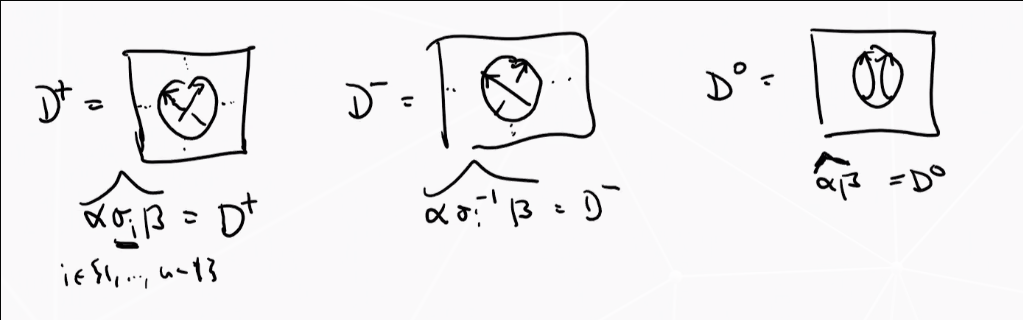
\includegraphics{figures/image_2020-07-10-11-40-29.png}

\begin{align*}
&a \tr_n \circ w_n(\alpha \sigma_1 \beta)- a\inv \tr_n \circ w_n (\alpha \sigma_i\inv \beta) - (v-v\inv) \tr_n \circ w_n(\alpha \beta) \\ \\
&= a \tr_n \qty{ w_n(\alpha) T_i w_n(\beta)} - a\inv \tr_n \qty{ w_n(a) T_i\inv w_n(\beta)} - (v-v\inv) \tr_n\qty{ w_n(\alpha) w_n(\beta)} \\ \\
&= \tr_n \qty{ a \qty{ w_n(\alpha) T_i w_n(\beta)} - a\inv \qty{ w_n(a) T_i\inv w_n(\beta)} - (v-v\inv) \qty{ w_n(\alpha) w_n(\beta)}} \\ \\
&= \tr_n\qty{ w_n(\alpha) \qty{ aT_i - a\inv T_i\inv - (v-v\inv)  }w_n(\beta) } \\ 
&= 0
.\end{align*}

\end{remark}

\hypertarget{categorifying-the-hecke-algebra}{%
\subsection{Categorifying the Hecke
Algebra}\label{categorifying-the-hecke-algebra}}

Idea: to categorify HOMFLY-PT, we will try to categorify the Hecke
algebra. This doesn't quite make sense yet: what does it mean to
categorify an entire algebra instead of just a number?

\begin{definition}[Additive Categories]

A category \(\mca\) is \emph{additive} iff

\begin{enumerate}
\def\labelenumi{\arabic{enumi}.}
\tightlist
\item
  The homs \(\mca(X, Y)\) is a \(\ZZ\dash\)module for all
  \(X, Y\in \mca\)
\item
  \(\mca(X, Y) \cross \mca(Y, Z) \to \mca(X, Z)\) where
  \((f, g) \mapsto g\circ f\) is \(\ZZ\dash\)bilinear.
\item
  \(\exists 0\in \mca\), an object that is both initial and terminal.
\item
  For all \(X, Y\in \mca\), there exists a coproduct \(X\oplus Y\)
\end{enumerate}

\end{definition}

\begin{definition}[Initial Objects]

Recall that an object \(I\) is initial in \(A\) iff for every \(X\)
there exists a unique \(I\to X\), and terminal iff there exists a unique
\(X\to I\).

\end{definition}

\begin{definition}[Coproduct]

Recall that a coproduct of \(X, Y\) is an object \(X\oplus Y\) with two
morphism \(\iota_X: X\to X\oplus Y, \iota_Y: Y\to X\oplus Y\) satisfying
the appropriate universal property.

\end{definition}

\begin{example}

\(R\dash\)bimodules over \(R\) a ring.

\end{example}

\begin{definition}[Essentially Small]

An additive category \(\mca\) is \emph{essentially small} iff the
isoclasses \([X]\) of objects form a set.

\end{definition}

\begin{definition}[Split Grothendieck Group]

Assume \(\mca\) is additive and essentially small. Then we can define a
free abelian group on
\begin{align*}
F(\mca) \definedas \theset{[X] \suchthat X\in \mca}
\end{align*} along with a subgroup
\begin{align*}
N(\mca) \definedas \theset{[X\oplus Y] - [X] - [Y]}
.\end{align*} Define the \emph{split Grothendieck group} as the
following:
\begin{align*}
K_0^\oplus \definedas F(A) / N(A)
\end{align*}

\end{definition}

\begin{remark}

Note that this starts to look like categorification: we can express
direct sums in terms of sums in a module. Notation: mod denotes finitely
generated, Mod denotes full categories.

\end{remark}

\begin{example}

\(\mca = k\dash\)mod, the category of finite-dimensional
\(k\dash\)vector spaces. There is a well-defined group morphism defined
on generators
\begin{align*}
\phi: F(\mca) &\surjects \ZZ \\
[V] &\mapsto \dim_k(V)
\end{align*} which is surjective since \(-[V]\) exists in the domain and
\([k^n] \mapsto n\) for all \(n\).

Note that this will factor through
\(K_0^\oplus(\mca) = F(\mca)/ N(\mca)\) via a map \(\bar\phi\) iff
\(N(\mca) \subseteq \ker \phi\). We can check
\begin{align*}
\phi\qty{[V\oplus W] - [V] - [W] } 
= \dim(V\oplus W) - \dim(V) - \dim(W) = 0
.\end{align*}

\begin{claim}

\(\phi\) is actually injective.

\end{claim}

\begin{proof}

Suppose
\begin{align*}
0 = \bar\phi\qty{ \sum \lambda_i [V_i]} = \sum \lambda_i \bar \phi([V_i]) = \sum \lambda_i \dim(V_i)
.\end{align*}

We can now check
\begin{align*}
\sum \lambda_i [V_i] = \sum \lambda_i \dim(V_i) [k] = [k] \sum \lambda_i \dim(V_i)
,\end{align*} where we use the fact that if \(\dim V = n\), then
\([V] = [k^n] = n[k]\).

\end{proof}

\end{example}

\begin{definition}[Categorification]

Let \(G\) be an abelian group, then \(\mca\) \textbf{categorifies} \(G\)
iff \(K_0^\oplus(\mca) \cong G\).

\end{definition}

\hypertarget{monday-july-13th}{%
\section{Monday July 13th}\label{monday-july-13th}}

\hypertarget{ring-structure-on-k_0oplusid.}{%
\subsection{\texorpdfstring{Ring structure on
\(K_0^\oplus(\id)\).}{Ring structure on K\_0\^{}\textbackslash oplus(\textbackslash id).}}\label{ring-structure-on-k_0oplusid.}}

\begin{definition}[Monoidal Categories]

A \emph{monoidal category} is a tuple
\((\mcc, \wait \tensor \wait, 1, \alpha, \ell, r)\) such that

\begin{itemize}
\tightlist
\item
  \(\mcc\) is a category
\item
  \(\wait \tensor \wait: \mcc \cross \mcc \to \mcc\) is a bifunctor.
\item
  \(1\in \mcc\)
\item
  Natural isomorphisms
  \begin{align*}
  \alpha_{X,Y,Z}: (X\tensor Y)\tensor Z \mapsvia{\cong} X\tensor (Y\tensor Z)
  \end{align*} for all \(X,Y,Z\in \mcc\) (associators).
\item
  Natural isomorphisms
  \begin{align*}
  \ell_X: 1\tensor X &\mapsvia{\cong} X\\
  r_X:X\tensor 1 &\mapsvia{\cong}X
  \end{align*} and for all \(X\in \mcc\).
\end{itemize}

Along with coherence axioms: for all \(W,X,Y,Z\in \mcc\),

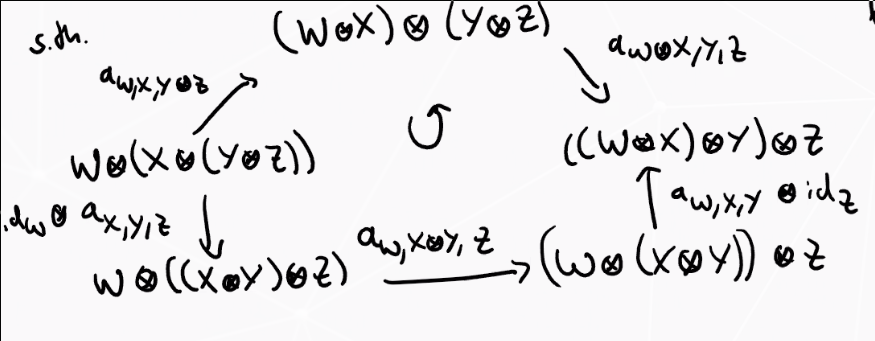
\includegraphics{figures/image_2020-07-13-11-09-53.png}

\begin{center}\includesvg[width=0.7\linewidth]{e973374a70b1566a28e5246fd442b871cbb8a3e2}\end{center}

\end{definition}

\begin{remark}

If \(\mcc\) is additive, we require \(\wait \tensor \wait\) to be
biadditive, i.e.~\(X\tensor \wait\) and \(\wait \tensor Y\) are additive
functors. In particular,
\begin{align*}
X\tensor (V\oplus W) \cong (X\tensor V) \oplus (X\tensor W)
\end{align*} and similarly
\begin{align*} 
(V\oplus W) \tensor Y \cong (V\tensor Y) \oplus (W\tensor Y)
.\end{align*}

\end{remark}

\begin{example}

\(\rmod\) with \(R\) a commutative unital ring, take
\(\tensor \definedas \tensor_R\) with \(1\) the ``regular left
\(R\dash\)module'' \({}_R R\) with \(R\) acting on the left by
multiplication. Similarly, \(R\dash\)bimodules, take \(1 = {}_R R_R\).

\end{example}

\begin{proposition}[?]

If \(\mca\) is additive and \((\mca, \tensor, 1, \alpha, \ell, r)\) is
monoidal, then setting \([X] \cdot [Y] \definedas [X\tensor Y]\) defines
a ring structure on \(K_0^\oplus(\mca) = F(\mca) / N(\mca)\).

\end{proposition}

\begin{proof}

\hfill

\begin{itemize}
\tightlist
\item
  This is well-defined on \(F(\mca)\).
\item
  Unital: Check \([X][1] = [X\tensor 1] = [X] = [1\tensor X] = [1][X]\)
\item
  Associativity:
  \begin{align*}
  ([X][Y])[Z] 
  &= [X\tensor Y][Z] \\
  &= [(X\tensor Y) \tensor Z]  \\
  &= [X\tensor (Y\tensor Z)]  \\
  &= [X][Y\tensor Z] = X([Y][Z])
  .\end{align*}
\item
  Distributive: Check.
\end{itemize}

Therefore \(F(\mca)\) is a unital ring.

\begin{itemize}
\tightlist
\item
  Check \(N(\mca) \subseteq F(\mca)\) is a two-sided ideal (use the
  isomorphism from the earlier remark.)
\end{itemize}

\end{proof}

\begin{example}

The group morphism \(\bar \phi: K_0^\oplus(\kmod) \mapsvia{\cong} \ZZ\)
is in fact a ring morphism.

\begin{itemize}
\tightlist
\item
  Check
  \begin{align*}
  \bar \phi([V][W]) 
  &= \bar\phi([V\tensor_k W]) \\
  &= \dim(V\tensor_k W) \\
  &= \dim(V) \dim(W) \\
  &= \bar\phi([V]) \bar\phi([W])
  .\end{align*}
\item
  Check \(\bar\phi([k]) = \dim k = 1\).
\end{itemize}

For \(\mca\) an additive category, for all \(i\in \ZZ\) there exist
additive functors

\begin{align*}
(i): \mca &\to \mca \\
X &\mapsto (i)(X) = X(i)
.\end{align*}

\end{example}

\begin{remark}

These satisfy \((j) \circ (i) = (i+j)\) and \((0) = \id_\mca\), so they
will correspond to degree shifts.

\end{remark}

\begin{proposition}[?]

Setting \(v^i[X] \definedas [X(i)]\) defines a
\(\ZZ[v, v\inv]\dash\)module structure on \(K_0^\oplus(\mca)\).

\end{proposition}

\begin{proof}

\hfill

\begin{itemize}
\item
  Check that this is well-defined on \(F(\mca)\); the module axioms will
  follow from the above remark.
\item
  Check that is descends to the quotient, i.e
  \begin{align*}
  v^i([X\oplus Y] -[X] - [Y])
  &= v^i]X\oplus Y - v^i[X] - v^i [Y] \\
  &= [(X\oplus Y)(i)] - [X(i)] - [Y(i)] \\
  &= [X(i)\oplus Y(i)] - [X(i)] - [Y(i)]
  .\end{align*}
\end{itemize}

\end{proof}

\begin{exercise}[?]

Show that \(K_0^\oplus(k\dash\text{grmod}) \cong \ZZ[v, v\inv]\) where
\([v] \mapsto \sum_{k\in \ZZ} \dim(V_n)v^n\) is an isomorphism of
\(\ZZ[v,v\inv]\dash\)modules (and in fact an isomorphism of
\(\ZZ[v,v\inv]\dash\)algebras).

\end{exercise}

\begin{remark}

For \((\mca, \tensor, 1, \alpha, \ell, r)\) a monoidal category with
additive functors \((i)\) as above, if
\begin{align*}
(i) \circ (X\tensor \wait) \cong (X\tensor \wait) \circ (i) \\
(i) \circ (\wait \tensor Y) \cong (\wait \tensor Y) \circ (i) 
\end{align*} using the fact that
\begin{align*}
(X\tensor Y)(i) \cong X \tensor (Y(i)) \cong (X(i)) \tensor Y
.\end{align*} Thus \(K_0^\oplus(\mca)\) is a
\(\ZZ[v, v\inv]\dash\)algebra.

\end{remark}

Recall that \(H_n^R(q, q-1)\) taking \(R = \ZZ[v, v\inv]\) with
\(q=v^{-2}\) and \(q-1 = z\) was the Iwahari-Hecke algebra, generated by
\(\theset{T_i}_{i\leq n-1}\) and the braid/skein relations.

Substitute \(Hs_i = vT_i\) (Soergel's correction) to obtain a new
presentation of \(H_n^{\ZZ[v, v\inv]}(v^{-2}, v^{-2}-1)\). The
generators are now \(\ts{ H_{s_i} \st i\leq n-1}\) and
\begin{align*}  
H_{s_i} H_{s_{i+1}} H_{s_i} 
&= H_{s_{i+1}} H_{s_i} H_{s_{i+1}} \\
H_{s_i} H_{s_j} 
&= H_{s_j}  H_{s_i} 
&& 
\abs{i-j} \geq 2 \\
H_{s_i}^2 
&= v^2 T_i^2 \\
&= v^2 \qty{ (v^{-2} - 1)T_i + v^{-2}1} \\
&= (1-v^{-2}) T_i + 1 \\
&= (v\inv - v) H_{s_i} +1
.\end{align*}

Notation: we'll abbreviate
\(\mch(S_n) = H_n^{\ZZ[v, v\inv]} (v^{-2}, v^{-2} - 1)\). There is a
standard basis
\begin{align*}  
H_w \definedas H_{s_{i_1}} \cdots H_{s_{i_r}} = v^{\ell(w)} T_w 
&&
w\in S_n,\,\, 
w = s_{i_1} \cdots s_{i_r}, \,\, 
\ell(w) = r
 .\end{align*} where \(w\) is written as a minimal length reduced
expression.

\hypertarget{some-technical-tools}{%
\subsection{Some technical tools}\label{some-technical-tools}}

\begin{enumerate}
\def\labelenumi{(\arabic{enumi})}
\tightlist
\item
  The Bruhat order.
\end{enumerate}

This is a partial order on the symmetric group \(S_n\) where
\(w'\leq w\) iff there exists a word for \(w'\) obtained by deleting
some \(s_i\) from the reduced expression for \(w\).

\begin{example}

For \(S_3\):

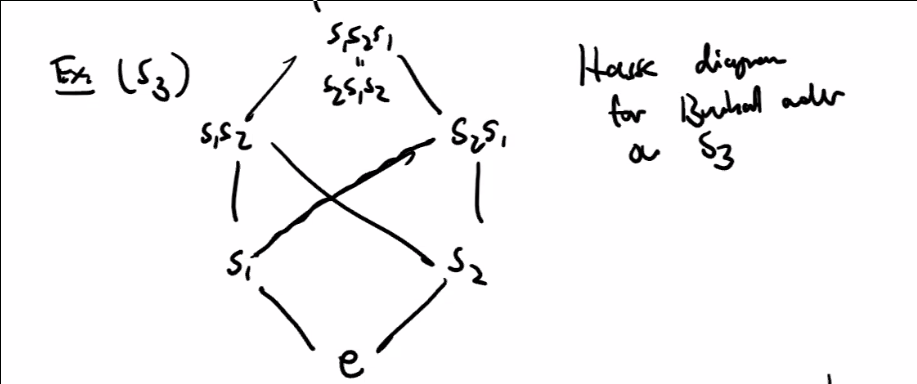
\includegraphics{figures/image_2020-07-13-11-54-42.png}

\end{example}

\begin{enumerate}
\def\labelenumi{(\arabic{enumi})}
\setcounter{enumi}{1}
\tightlist
\item
  The Bar involution.
\end{enumerate}

There is a ring morphism
\begin{align*}
\mch(S_n) &\to \mch(S_n) \\
h &\mapsto \bar h
.\end{align*} uniquely determined by \(\bar{H_{s_i}} = H_{s_i\inv}\)
(which incidentally equals \(H_{s_i} + (v-v\inv)1\)) and
\(\bar v = v\inv\).

\begin{theorem}[KL-Soergel]

For all \(w\in S^n\) there exists a unique \(C_w \in \mch(S_n)\) such
that

\begin{enumerate}
\def\labelenumi{\arabic{enumi}.}
\tightlist
\item
  \(\bar{C_w} = C_w\), self-duality
\item
  \(C_w = H_w + \sum_{x < w} h_{x, w} H_x \in v\ZZ[v]\), upper
  triangularity.
\end{enumerate}

\end{theorem}

\begin{definition}[?]

\(\theset{C_w \suchthat w\in S_n}\) is the \emph{KL-basis} of
\(\mch(S_n)\).

\end{definition}

This is a basis because we can refine \(\leq\) to a total order, then
write a change-of-basis matrix from the standard basis to this:

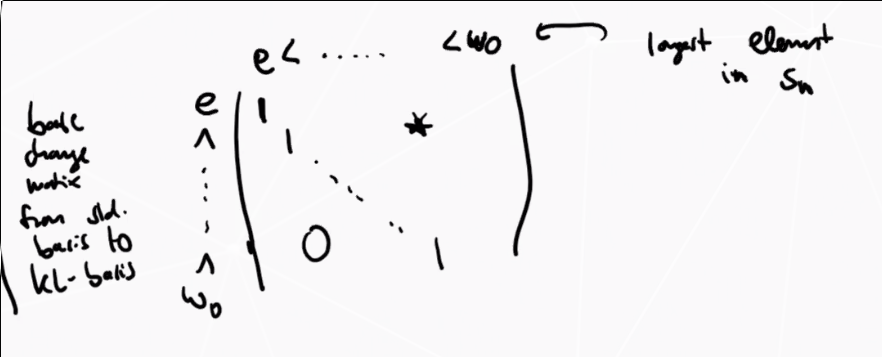
\includegraphics{figures/image_2020-07-13-11-59-25.png}

The elements \(h_{x, w} \in \ZZ[v, v\inv]\) are called the
\emph{KL-polynomials} where we set \(h_{w, w} = 1\) and \(h_{x, w} = 0\)
when \(x\not\leq w\).

\begin{example}

Note \(C_e = H_e\) and
\begin{align*}  
C_{s_1} &= H_{s_1} + v1 \\
C_{s_2} &= H_{s_2} + v1
.\end{align*}

Thus (2) is satisfied, and (1) follows from
\begin{align*}
\bar{C_{s_i}} 
&= \bar{H_{s_i} + v_1} \\
&= \bar{H_{s_1}} + \bar{v} 1 \\
&= H_{s_i\inv} + v\inv 1 \\
&= H_{s_i} + (v-v\inv)1 + v\inv 1 \\
&= H_{s_i} + v1
.\end{align*}

Can also check that
\begin{align*}
C_{s_1 s_2} &= C_{s_1 s_2} 
&&\text{automatically self-dual} \\
&= (H_{s_1} + v) (H_{s_2} + v) \\
&= H_{s_1} H_{s_2} + v H_{s_2} + vH_{s_1} + v^2
.\end{align*}

Similarly expand
\(C_{s_2 s_1} = H_{s_2 s_1} + vH_{s_1} + vH_{s_2} + v^2\).

Finally compute

\begin{align*}
C_{s_2} C_{s_1} C_{s_2} 
&= (H_{s_2 s_1} +v H_{s_1} + vH_{s_2} + v^2 )(H_{s_2} + v) \\
&= H_{s_2 s_1 s_2} + v H_{s_1 s_2} + v H_{s_2}^2 + v^2 H_{s_2} = v H_{s_2 s_1} + v^2 H_{s_1} + v^2 H_{s_2} + v^4
.\end{align*}

Note that coefficients need to be contained in \(v\ZZ[v]\) but we still
need self-duality.

\end{example}

\hypertarget{tuesday-july-14th}{%
\section{Tuesday July 14th}\label{tuesday-july-14th}}

\begin{remark}

\hfill

\begin{itemize}
\tightlist
\item
  The KL basis can be complicated -- you can compute them recursively,
  but may need to subtract off ``constant coefficients'' to obtain
  self-dual elements.
\item
  There are no closed formulas in general.
\item
  For any \(P\in ! + q \ZZ^{\geq 0}[q]\) there exists an \(m\in \ZZ\)
  such that \(v^m P(v^{-2})\) occurs as a KL-polynomial.
\item
  \textbf{The KL Positivity Conjecture}:
  \(h_{x, w} \in \ZZ^{\geq 0} [v]\), and in fact these non-negative
  coefficients can be realized as the graded dimension of the local
  intersection cohomology of Schubert varieties.
\end{itemize}

\end{remark}

\hypertarget{why-care-about-kl-positivity}{%
\subsection{Why care about KL
Positivity?}\label{why-care-about-kl-positivity}}

Set
\begin{align*}
\lieg = \liesl(n, \CC) = \theset{A\in \CC^{n\times n} \suchthat \tr(A) = 0}\\
\text{with } 
[AB] = AB - BA
.\end{align*}

The case of finite-dimensional representations is well understood, since
everything decomposes into simple modules. In the infinite case, we
consider the principal block of category \(\OO\), denoted
\(\OO_0(\lieg)\).

There is a correspondence

\begin{center}\includesvg[width=0.7\linewidth]{0bdad2c6e53d3b43d47858c0e87d87fad6ae383f}\end{center}

The \textbf{KL-multiplicity conjecture} states
\begin{align*} 
[\Delta(w) : L(x)] = h_{x, w}(1)
,\end{align*} where the LHS counts how often \(L(x)\) occurs as a
subquotient in a composition series for \(\Delta(w)\). Determining the
characters \(\ch L(w)\) can be done using translation functors, and
corresponds to determining the characters of all simple highest weight
modules (not necessarily finite-dimensional), and is a vast
generalization of Weyl's character formula.

This was the birth of geometric representation theory, and the proof
involved \(D\dash\)modules, perverse sheaves, and Deligne's proof of the
Weil conjectures.

\textbf{Goal}: categorify \(\mch_n(S_n)\), the associative unital
\(\ZZ[v, v\inv]\dash\)algebra given by
\(\gens{\theset{H_i \suchthat i\leq n-1}}\) subject to
\begin{align*}
H_{s_{i+1}}
H_{s_{i}}
H_{s_{i+1}} &= 
H_{s_{i+1}}
H_{s_{i}}
H_{s_{i+1}} \\
H_{s_{i}}
H_{s_{j}}
&=
H_{s_{j}}
H_{s_{i}} 
&& \abs{i-j} \geq 2 \\
H_{s_{i}}^2 &= (v\inv - v) H_{s_i} + 1
.\end{align*}

Or equivalently, setting \(C_{s_i} = H_{s_i} + v\),
\begin{align*}
C_{s_{i+1}}
C_{s_{i}}
C_{s_{i+1}}  + C_{s_i} &= 
C_{s_{i+1}}
C_{s_{i}}
C_{s_{i+1}} + C_{s_{i+1}} \\
C_{s_{i}}
C_{s_{j}}
&=
C_{s_{j}}
C_{s_{i}}  
&&\abs{i-j} \geq 2 \\
C_{s_{i}}^2 
&= (v\inv - v) H_{s_i} + 1
.\end{align*}

\begin{remark}

The presentation above can be ``lifted'' to a categorical level. So we
want to find a category \(\mca\) which is additive, monoidal, graded,
and abelian such that

\begin{itemize}
\tightlist
\item
  \(K_0^\oplus(\mca) \cong H(S_n)\) is an isomorphism of
  \(\ZZ[v, v\inv]\dash\)algebras.
\item
  There are objects \(B_{s_i}\) such that
\end{itemize}

\begin{align*}  
1. && B_{s_i} \tensor B_{s_i} &\cong B_{s_i}(1) \oplus B_{s_i}(-1) \\
2. && B_{s_j} \tensor B_{s_i} &\cong B_{s_i} \tensor B_{s_j} && \text{ for } \abs{i-j} \geq 2 \\
3. && B_{s_i} \tensor B_{s_{i+1}} \tensor B_{s_i} \oplus B_{s_{i+1}} &\cong B_{s_{i+1}} \tensor B_{s_{i}} \tensor B_{s_{i+1}} \oplus B_{s_{i}}
.\end{align*}

\end{remark}

Question 1: What are the objects \(B_{s_i}\)? Set
\(R = \CC[x_1, \cdots, x_n]\) with \(\abs{x_i} = 2\), yielding a graded
\(\CC\dash\)algebra where \(s_i\) permutes \(x_i, x_{i+1}\). We can look
at the invariant ring,
\begin{align*}
R^{s_i} \definedas \theset{f\in R \suchthat s_i f = f}
\end{align*} and note that \(R\) and any of its shifts are modules over
this ring. So set,
\begin{align*}
B_{s_i} \definedas R \tensor_{R^{s_i}} R(-1)
\end{align*} which is a graded \(R\dash\)bimodule.

\begin{proposition}[?]

We have an isomorphism of \(R\dash\)bimodules satisfying the desired
relations.

\end{proposition}

\begin{claim}

\(R\cong R^{s_i}(2) \oplus R^{s_i}\) as graded
\(R^{s_i}\dash\)bimodules.

\end{claim}

\begin{proof}

It suffices to show that every \(f\in R\) can be written uniquely as
\begin{align*}
f = g(x_i - x_{i+1}) + h  \text{  with } g, h \in R^{s_i}
.\end{align*}\\

\textbf{Uniqueness}: If \(f =g'(x_i - x_{i+1}) + h'\) then
\begin{align*}
g'(2x_i - 2x_{i+1}) 
&= f - s_i f \\
&= g(x_i - x_{i+1}) - g(x_{i+1} - x_i)  \\
&= g(x_i - x_{i+1} - x_{i+1} + x_i) \\
&= g(2x_i - 2x_{i+1})
.\end{align*}

Since this is an integral domain, \(g=g'\), and
\begin{align*}
h = f - g (x_i - x_{i+1}) = f - g'(x_i - x_{i+1}) = h'
.\end{align*}

\textbf{Existence}: \(x_k \in R^{s_i}\) is \(s_i\) invariant if
\(k\neq i, i+1\), and
\begin{align*}
x_i = {1\over 2}\qty{ x_i - x_{i+1}} + {1\over 2}\qty{x_i + x_{i+1}} \in R^{s_i} \qty{\cdots} + R^{s_i}  \\
x_{i+1} = -{1\over 2}\qty{ x_i - x_{i+1}} + {1\over 2}\qty{x_i + x_{i+1}} \in R^{s_i} \qty{\cdots} + R^{s_i}  \\
.\end{align*}

So every \(f\in R\) can be expressed as a polynomial in
\(x_i - x_{i+1}\) with coefficients in \(R^{s_i}\). Since
\(\qty{x_i - x_{i+1}}^2 \in R^{s_i}\), any polynomial in
\(x_i - x_{i+1}\) with coefficients in \(R^{s_i}\) can be written as
\(g(x_i - x_{i+1}) + h\) with \(g, h \in R^{s_i}\). This proves the
claim.

We can now check
\begin{align*}
B_{s_i} \tensor_R B_{s_i} 
&=
\qty{R \tensor_{R^{s_i}} R} \tensor_R 
\qty{R \tensor_{R^{s_i}} R}(-2) \\
&\cong R \tensor_{R^{s_i}} R \tensor_{R^{s_i}} R(-2) \\
&\cong R \tensor_{R^{s_i}} \qty{ R^{s_i}(2) \oplus R^{s_i}  } \tensor_{R^{s_i}} R(-2) \\
&\cong R \tensor_{R^{s_i}} \qty{ R^{s_i}(2)   } \tensor_{R^{s_i}} R(-2)  \oplus
R \tensor_{R^{s_i}} \qty{ R^{s_i}  } \tensor_{R^{s_i}} R(-2) \\
&\cong R \tensor_{R^{s_i}} R \oplus R\tensor_{R^{s_i}} R(-2) \\
&\cong B_{s_i}(1) \oplus B_{s_i}(-1)
.\end{align*}

\end{proof}

\hypertarget{soergels-dream}{%
\subsection{Soergel's Dream}\label{soergels-dream}}

Come up with a purely algebraic proof of the KL conjecture (without
using machinery from geometric representation theory). Consider the
center of category \(O\), \(Z(\OO_0)\), the endomorphism ring of the
identity functor. It can be shown that this is isomorphic to the
coinvariant ring
\(\CC[x_1, \cdots, x_{n+1}] / \CC[x_1, \cdots, x_{n+1}]^{S^n}\). Thus
invariant theory is ``hidden'' in the category \(\OO_0(\lieg)\).

\begin{quote}
Proved originally, but used some decomposition theory. Recent proof from
Elias Williams? Using hodge structures.
\end{quote}

\textbf{Question}: What is the category \(\mca\)?

\begin{definition}[Bott-Samelson Bimodules]

Take \(R\dash\grdim\), the category of graded \(R\dash\)bimodules, which
is finitely generated as both left/right \(R\dash\)modules. This is
additive, monoidal, and graded, but this category is too big. So we
carve out a smaller subcategory.

For \(w\in S_n\), write the formal word
\(\bar w = s_{i_1} \cdots s_{i_r}\) a reduced expression for \(w\). Note
that this depends on which reduced expression is used. Now define
\begin{align*}
BS(\bar w) 
&\definedas \bigotimes^{j\leq r}{}_{R^{s_{i_j}}} \,\,B_{s_{i_j}}  && BS(\emptyset) = R \\
&\cong R \tensor_{R^{s_{i_1}}} R \tensor \cdots \tensor_{R^{s_{i_r}}} R
\end{align*} where the isomorphism is canonical. This is the
\textbf{Bott-Samelson bimodule}.

\end{definition}

\begin{definition}[?]

\hfill

\begin{itemize}
\tightlist
\item
  A Soergel bimodule is a direct summand of a finite sum of grading
  shifts of Bott-Samelson bimodules.
\item
  The category \(\mathbf{SBim}\) of Soergel bimodules is the strictly
  full subcategory of \(R\dash\grdim\) consisting of Soergel bimodules.
\item
  Equivalently, the smallest full subcategory of \(R\dash\grdim\)
  consisting of \(R, B_{s_i}\) and closed under
  \(\tensor_R, \oplus, (i)\) and taking direct summands.
\end{itemize}

\end{definition}

\begin{remark}

The category \(\mathbf{SBim}\) is additive, monoidal, and graded, but
\textbf{not} abelian.

\end{remark}

\begin{definition}[Indecomposable]

Recall that a module \(X\) is \textbf{indecomposable} \(\iff\)
\(X \cong A\oplus B\) implies \(A\cong 0\) or \(B\cong 0\).

\end{definition}

\begin{definition}[Krull-Schmidt]

A category \(\mathcal{C}\) is \textbf{Krull-Schmidt} \(\iff\) every
object decomposes uniquely into a \emph{finite} direct sum of
indecomposable objects.

\end{definition}

\begin{theorem}[?]

\hfill

\begin{enumerate}
\def\labelenumi{\arabic{enumi}.}
\tightlist
\item
  \(\mathbf{SBim}\) is \emph{Krull-Schmidt}.
\end{enumerate}

\begin{quote}
Note that such uniqueness here means that if
\(\bigoplus_{i=1}^r X_i \cong \bigoplus_{i=1}^s Y_i\) then \(r=s\) and
there is some permutation \(\pi \in S_r\) such that
\(X_{\pi(i)} \cong Y_i\).
\end{quote}

\begin{enumerate}
\def\labelenumi{\arabic{enumi}.}
\setcounter{enumi}{1}
\tightlist
\item
  There is a bijection
  \begin{align*}
  S_n &\tofrom \correspond{\text{Indecomposable Soergel bimodules} }/ \text{\tiny Isomorphism and shifts} \\
  w &\mapsto B_w
  .\end{align*}
\end{enumerate}

Moreover \(\theset{ S[B_w] \suchthat w\in S_n }\) form a basis of
\(K_0^\oplus(\mathbf{SBim})\) as \(\ZZ[v, v\inv]\dash\)modules.

\begin{enumerate}
\def\labelenumi{\arabic{enumi}.}
\setcounter{enumi}{2}
\tightlist
\item
  There is a \(\ZZ[v, v\inv]\dash\)algebra morphism
  \begin{align*}
  c: \mch(S_n) &\mapsvia{\cong} K_0^\oplus(\mathbf{SBim}) \\
  C_{s_i} &\mapsto [B_{s_i}]
  .\end{align*}
\end{enumerate}

\end{theorem}

\begin{remark}

This implies both the KL positivity and multiplicity conjectures. The KL
basis corresponds to the basis given by the indecomposable Soergel
bimodules.

\end{remark}

\hypertarget{wednesday-july-15th}{%
\section{Wednesday July 15th}\label{wednesday-july-15th}}

Let \(R\) be a unital (not necessarily commutative) ring, then we can
consider two categories:

\begin{itemize}
\tightlist
\item
  \(\rmod\): the category of left \(R\dash\)modules
\item
  \(\modr\): the category of right \(R\dash\)modules
\end{itemize}

Let \(X\in \modr\) a consider the functor
\begin{align*}
X\tensor_R \wait: \rmod &\to \ZZ\dash\text{mod} \\
Y &\mapsto X\tensor_R Y
.\end{align*} Given a short exact sequence, we obtain a right-exact
sequence, i.e.~this functor is right-exact

\begin{warning}

The induced map \(X\tensor_R A \to X\tensor_R B\) need not be injective.

\begin{center}\includesvg[width=0.7\linewidth]{d8b2d2578c385e03b869df5715e1d806a9b80d59}\end{center}

\end{warning}

Then \(f_*\) is not injective, since
\(\qty{\id \tensor_\ZZ (\cdot 2)} (T\tensor 1)) = T\tensor 2 = 2T\tensor 1 = 0\).

Recall that this has derived functors \(\tor_i^R(X, \wait)\) which
vanish if either component is projective and yields a LES.

\begin{definition}[Flat Modules]

An \(R\dash\)module \(X\) is \emph{flat} if \(X\tensor_R \wait\) is
exact.

\end{definition}

Recall that free \(\implies\) projective \(\implies\) flat.

Construction of \(\tor_i^R(X, Y)\):

\begin{enumerate}
\def\labelenumi{\arabic{enumi}.}
\item
  \(\rmod\) has enough projectives, so take a projective resolution of
  \(Y\):
  \begin{align*} 
  P_* \da \qty{ \cdots \to P_2 \to P_1 \to P_0 \to Y \to 0 }
  \end{align*} with each \(P_j\) projective.
\item
  Apply \(X\tensor_R \wait\) to \(P_*\):
  \begin{align*}
  X\tensor_R \wait P_\wait: \cdots \to X \tensor_R P_2 \to X\tensor_R P_1 \to X\tensor_R P_0 \to 0
  .\end{align*} Note that this is a chain complex, but not exact in
  general.
\item
  Define
  \begin{align*}
  \tor_i^R(X, Y) \definedas H_i(X\tensor_R P_\wait)
  ,\end{align*} i.e.~take kernels mod images.
\end{enumerate}

Note that choices were made, is this independent (up to natural
isomorphism) of the chosen projective resolution \(P_\wait\)?

\begin{lemma}[?]

Let \(f: Y\to Y' \in \rmod\), and let \(P_\wait, P_\wait'\) be
respective projective resolutions. Then there exists a map of chain
complexes \(\tilde f: P_\wait \to P_\wait'\) such that

\begin{center}\includesvg[width=0.7\linewidth]{612f4e0b31803c1155042523fc02b896afb2091e}\end{center}

where all of the squares commute, and \(\tilde f\) is unique up to chain
homotopy.

\end{lemma}

So take \(f = \id_Y: Y\to Y\), by the lemma there is a map of chain
complexes \(\tilde \id: P_\wait \to P_\wait'\), and applying
\(X\tensor_R \wait\) yields a map of chain complexes
\(X\tensor_R P_\wait \to X\tensor_R P_\wait'\). Since homotopic maps
yield the same map in homology, we get maps
\(H_i(X\tensor_R P_\wait) \to H_i(X\tensor_R P_\wait')\), and it can be
checked that these maps are isomorphisms for every \(i\) by using the
lemma again but reversing all of the maps.

\begin{remark}

For \(A\in \text{mod}\dash\ZZ\), \(A\) is torsionfree
\(\iff \tor_1^\ZZ(A, B) = 0\) for every other
\(B\in \ZZ\dash\text{mod}\). As a special case, for \(k\) a field and
\(R\) a \(k\dash\)algebra, \(R\tensor_k R\op\) is a \(k\dash\)algebra
when equipped with the product
\((a\tensor b)\cdot(a'\tensor b') = (aa') \tensor (bb')\). This is
called the \textbf{enveloping algebra} of \(R\)

\begin{quote}
Note: has nothing to do with universal enveloping algebras in Lie
theory.
\end{quote}

There is an isomorphism of categories
\begin{align*}
R\tensor_R R\op\dash\text{mod} &\mapsvia{\cong} R\dash\text{bimod} \\
(r_1\tensor r_2) \cdot m &\mapsfrom
r_1 \cdot m \cdot r_2 \in RMR 
.\end{align*}

The point of this is that we may not be able to make sense of projective
resolutions on the RHS, but we can think of them as usual modules over
the enveloping algebra instead.

\end{remark}

\begin{warning}

Some care must be taken with the monoidal structure. The monoidal
structur in the LHS is \(\tensor_{R\tensor_R R\op}\), whereas it is
\(\tensor_R\) in the RHS.

\end{warning}

\begin{definition}[Hochschild Homology]

Define the \(i\)th \textbf{Hochschild homology} of \(R\) as the functor
\begin{align*}
HH_i(R, \wait) \definedas \tor_i^{R\tensor_R R\op}(R, \wait) : R\dash\text{Bimod} &\to k\dash\text{mod}
.\end{align*}

\end{definition}

\begin{remark}

Note that this lands in \(k\dash\)modules instead of
\(\ZZ\dash\)modules. Moreover, everything works in the graded setting
and yields a functor \(R\dash\text{grBimod} \to k\dash\text{grMod}\).

\end{remark}

How does this relate to the HOMFLY-PT polynomial? Recall that we had a
trace
\begin{align*} 
\mch(S_n) \mapsvia{\tr}  \ZZ[ v, v\inv]
,\end{align*} and we think of \(HH\) as the categorification of the
trace on the Hecke algebra. It has trace-like behavior, namely
\begin{align*}
HH_\wait(R, M\tensor_R N) \cong HH_\wait(R, N\tensor_R M) \quad \in k\dash\text{Mod}
,\end{align*} which is similar to \(\tr(ab) = \tr(ba)\).

\begin{example}

Consider \(HH_\wait(\CC[t], \CC[t])\) with \(\abs t = 2\).

\begin{enumerate}
\def\labelenumi{\arabic{enumi}.}
\tightlist
\item
  Write a free resolution of \(\CC[t]\) as a
  \(\CC[t] \tensor_\CC \CC[t]\dash\)module:

  \begin{center}\includesvg[width=0.7\linewidth]{d1a53c0c76cb5b14892eae3cc233bc422b097552}\end{center}
\item
  Apply \(\CC[t] \tensor_{\CC[t] \tensor_\CC \CC[t]} \wait\).

  \begin{center}\includesvg[width=0.7\linewidth]{802e475bd0667b1900a4ceb02c525ff557d43ac8}\end{center}
\end{enumerate}

Note that the image is equal to
\begin{align*}
f \tensor (tg\tensor h) \cdot (1\tensor 1) - f\tensor (g\tensor th)\cdot (1\tensor 1) = 
tgfh \tensor 1\tensor 1 - gfth \tensor 1 \tensor 1 = 0
,\end{align*} so this is in fact the zero map.

We thus have

\begin{center}\includesvg[width=0.7\linewidth]{01aea8476e6c60d910d6f9b8711e60692145ee15}\end{center}

\begin{enumerate}
\def\labelenumi{\arabic{enumi}.}
\setcounter{enumi}{2}
\tightlist
\item
  Read off
  \begin{align*}  
  HH_0(\CC[t], \CC[t]) &\cong \CC[t] \\
  HH_1(\CC[t], \CC[t]) &\cong \CC[t](2)
  .\end{align*}
\end{enumerate}

\end{example}

\newpage

\newpage
\section{Indices}
\listoftodos[List of Todos]

% Hook into amsthm environments to list them.
\renewcommand{\listtheoremname}{Definitions}
\listoftheorems[ignoreall,show={definition}, numwidth=3.5em]

\renewcommand{\listtheoremname}{Theorems}
\listoftheorems[ignoreall,show={theorem,proposition}, numwidth=3.5em]

\renewcommand{\listtheoremname}{Exercises}
\listoftheorems[ignoreall,show={exercise}, numwidth=3.5em]

\listoffigures


\printbibliography[title=Bibliography]


\end{document}
